\documentclass[12pt]{article}

\usepackage[T1]{fontenc}
\usepackage{lmodern}
\usepackage[left=2cm,right=2cm,top=2cm,bottom=3cm]{geometry}
\usepackage{graphicx}
\usepackage{tikz}
\usetikzlibrary{shapes,backgrounds,calc,arrows,arrows.meta,patterns,matrix,positioning}
\usepackage{amsmath}
\usepackage{booktabs}
\usepackage{xcolor}
\usepackage{pgfplots}
\pgfplotsset{compat=1.18}
\usepgfplotslibrary{groupplots}
\usepackage{listings}
\usepackage{float}
\usepackage{tabularx}
\usepackage[setpagesize=false,colorlinks=true,linkcolor=blue,urlcolor=red,
  pdftitle={Adaptive Data Profiling with ML-Based Quality Checks for ETL Pipeline Quality and Cost Optimization},
  pdfauthor={Koorosh Komeili Zadeh}]{hyperref}
\frenchspacing
\setlength{\parindent}{0pt}
\setlength{\parskip}{8pt}

% ── Colour palette ───────────────────────────────────────────────────────────
\definecolor{leidenblue}{RGB}{0,46,104}
\definecolor{recall}{RGB}{22,163,74}
\definecolor{precision}{RGB}{37,99,235}
\definecolor{f1color}{RGB}{234,88,12}
\definecolor{colorgray}{RGB}{156,163,175}
\definecolor{codebg}{RGB}{248,250,252}
\definecolor{codeborder}{RGB}{203,213,225}
\definecolor{keywordcolor}{RGB}{124,58,237}
\definecolor{stringcolor}{RGB}{220,38,38}
\definecolor{commentcolor}{RGB}{107,114,128}

% ── YAML listing style ───────────────────────────────────────────────────────
\lstdefinelanguage{yaml}{
  keywords={true,false,null},
  keywordstyle=\color{keywordcolor}\bfseries,
  basicstyle=\ttfamily\small,
  sensitive=false,
  comment=[l]{\#},
  commentstyle=\color{commentcolor}\itshape,
  stringstyle=\color{stringcolor},
  morestring=[b]',
  morestring=[b]",
}
\lstset{
  language=yaml,
  backgroundcolor=\color{codebg},
  frame=single,
  framerule=0.8pt,
  rulecolor=\color{codeborder},
  xleftmargin=12pt,
  xrightmargin=4pt,
  framexleftmargin=8pt,
  aboveskip=10pt,
  belowskip=4pt,
  showstringspaces=false,
  breaklines=true,
  captionpos=b,
  numbers=none,
}

\makeatletter
\newcommand{\supervisor}[1]{\gdef\@supervisor{#1}}
\newcommand{\@supervisor}{}
\makeatother

\makeatletter
\newcommand{\secondsupervisor}[1]{\gdef\@secondsupervisor{#1}}
\newcommand{\@secondsupervisor}{}
\makeatother

\makeatletter
\newcommand{\studentnumber}[1]{\gdef\@studentnumber{#1}}
\newcommand{\@studentnumber}{}
\makeatother

\makeatletter
\newcommand{\thesistype}[1]{\gdef\@thesistype{#1}}
\newcommand{\@thesistype}{}
\makeatother

\makeatletter
\newcommand{\studyprogram}[1]{\gdef\@studyprogram{#1}}
\newcommand{\@studyprogram}{}
\makeatother

% Redefine maketitle
\makeatletter
\renewcommand{\maketitle}{
  \begin{titlepage}

    \thispagestyle{empty}

    \vspace{1cm}

    \noindent
    \includegraphics{logoleiden} \\
    \vspace{1cm}
    
    % Title
    \noindent {\Huge\bfseries \@title \par}

    \vspace{2cm}

    \noindent % Author
    {\Large \@author ~(\@studentnumber) \par}

    \vfill

    \begin{large}

    \noindent Supervisors:\\
    \noindent { \@supervisor ~\& \@secondsupervisor \par}

    \vspace*{2.8cm}
    \noindent \textsc{\@thesistype -- \@studyprogram}

    \vspace*{5mm}
    \noindent Leiden Institute of Advanced Computer Science (LIACS) \\
    \url{liacs.leidenuniv.nl}  \hfill {\large \@date \par}

    \end{large}

\newpage

  \end{titlepage}
}
\makeatother

\title{Adaptive Data Profiling with ML-Based Quality Checks for ETL Pipeline Quality and Cost Optimization}
\author{Koorosh Komeili Zadeh}
\studentnumber{s3893995}
\date{\today}
\supervisor{Joost Visser}
\secondsupervisor{Jan van Rijn}
\thesistype{Bachelor Thesis}
\studyprogram{Data Science and Artificial Intelligence}

\begin{document}
\hypersetup{pageanchor=false}
\maketitle
\hypersetup{pageanchor=true}
\pagenumbering{roman}

\thispagestyle{empty}
\begin{abstract}
\noindent
\textbf{Background.} Data pipelines rely on simple rule-based quality checks to ingest, process, and store data in businesses. These traditional checks often fail to detect source-level semantic errors such as outliers before data reaches downstream users.

\noindent
\textbf{Aim.} This thesis investigates whether automated learning-based anomaly detection is a reliable, low-cost addition to rule-based quality checks in the ingestion layer of ETL pipelines.

\noindent
\textbf{Method.} We designed and implemented a modern ETL pipeline to evaluate a production-ready library developed for this purpose. The pipeline simulates a real-world data ingestion process on hourly weather data with injected controlled anomalies to provide ground-truth labels for effectiveness evaluation and computational overhead measurement. We compared both automated anomaly-detector selection (AutoML) and automated neural architecture search (Auto-NN) as approaches to automated learning-based detection.

\noindent
\textbf{Results.} AutoML reliably detected anomalies on stable columns at low computational cost. Compared to Auto-NN, it ran 9.13$\times$ faster and achieved a 4.1$\times$ higher mean F2 score. Neural models added complexity without improving detection.

\noindent
\textbf{Conclusion.} AutoML-based data profiling is a practical addition to ETL pipelines. Detection quality and computational cost depend strongly on the nature of the upstream data, making adaptive profiling a natural fit for some sources and impractical for others.
\end{abstract}


\newpage
\thispagestyle{empty}
\tableofcontents
\thispagestyle{empty}
\clearpage
\pagenumbering{arabic}

% ============================================================
\section{Introduction}\label{sec:introduction}
% ============================================================

In data-driven organizations, data is collected from multiple distributed sources and must be processed, transformed, and stored before it can support dashboards, analytics, and business decisions \cite{munappy2020datapipeline}. Engineers manage this flow using automated systems called data pipelines, which define where data is collected, how it is processed, and where it is stored.

The most common type is the ETL pipeline: Extract, Transform, Load. Data is pulled from an upstream source, processed, transformed, aggregated, and then written to a data warehouse where analysts and downstream users can use it.

The problem is that traditional quality checks inside ETL pipelines are rule-based. A data engineer writes checks like ``temperature must not be null'' or ``pressure must be an integer type between 870 and 1085 hPa.'' These rules work well for obvious errors, but they only catch problems the engineer already knew about. Statistical anomalies, gradual sensor drift, or unexpected value distributions can pass through rule checks without triggering any alert \cite{chu2016datacleaning, Maddali2021AutomatingDQ}.

This thesis investigates whether machine learning can address this limitation. Instead of fixed rules, a model learns what normal data looks like from historical data and flags anything that deviates from that learned pattern, for example, a temperature reading that passes a valid-range check but sits far outside the recent seasonal norm. The goal is to make this automatic, requiring no manual rule-writing and minimal domain expertise for individual columns.

\subsection{Motivation and Practical Relevance}

Rule-based quality checks exist, but subtle anomalies still pass through pipelines unnoticed. Quality checks are often applied after data has already been processed, so problems reach analytics and models before anyone spots them.

Recent industry work \cite{databricks2025aietl} shows that AI-driven ETL systems can automatically learn what normal data looks like and detect deviations before they reach downstream systems. Problems get caught earlier, before they propagate.

One main motivation is the principle of shift-left data quality: validating data as early as possible in the pipeline, ideally at the point of ingestion \cite{datakitchen2023shiftleft}. If a bad record enters at the point of ingestion, every transformation that follows inherits the defect. Without early validation, each downstream system encounters and addresses the same issue independently, compounding both effort and cost.

The other motivation is to reduce the cost of computation for high-quality data delivery by applying outlier detection once, rather than repeatedly by different downstream users. In practice, many data teams skip anomaly detection entirely due to the engineering effort and domain expertise required.
\subsection{Research Questions}

The main research question is:

\begin{center}
\emph{How effective and practical is learning-based anomaly detection as an addition to rule-based quality checks in ETL pipeline ingestion?}
\end{center}

This is explored through three sub-questions:

\begin{itemize}
  \item In terms of \emph{effectiveness}: 
  
  How accurately can learning-based anomaly detection identify outlier data quality issues compared to rule-based checks?
  \item In terms of \emph{practicality}:

  What is the computational overhead of integrating learning-based anomaly detection into the ingestion stage, and how does it scale with data size?
  \item In terms of \emph{learning model}:
  
  Does machine learning outperform neural architecture search in the trade-off between detection accuracy and computational cost for automated anomaly detection?
\end{itemize}

Throughout this thesis, the term \textbf{adaptive data profiling} refers to a per-column quality check layer that trains a statistical anomaly detection model on each column's own historical data. It is adaptive in that the algorithm selected varies per column based on its data characteristics, each upstream source trains its own model, and the models can be retrained on a schedule as data patterns change over time.

% ============================================================
\section{Background}\label{sec:background}
% ============================================================

\subsection{Data Pipelines in Practice}

A data pipeline is the system that handles this automatically. There are two main types. Real-time pipelines process data as it arrives, suitable for fraud detection or live dashboards. ETL pipelines process data in batches on a schedule, suitable for analytics, reporting, and training machine learning models.

\subsubsection{Business Use of ETL Pipelines}

ETL pipelines are central to how data-driven companies operate. A travel platform such as Skyscanner might collect different types of data that affect flight pricing, for example:

\begin{itemize}
  \item Data from booking platforms such as Booking.com to identify demand based on hotel reservations.
  \item Data from airlines such as KLM and Lufthansa to adjust pricing and identify travel seasons.
  \item Data from weather services to predict when people are more likely to travel to destinations with optimal weather.
\end{itemize}

This data can be used to adjust prices based on demand, helping the company remain profitable, stay competitive in the market, and offer customer-friendly prices. This process can be automated through data pipelines.

In each case, the pipeline extracts raw data from sources the company does not control, transforms it into a consistent and usable format, and loads it into a warehouse that supports products and business decisions. The quality of everything downstream depends directly on the quality of the data that flows through the pipeline.

\subsubsection{ETL: Extract, Transform, Load}

\textbf{Extract} pulls data from a source: a REST API, a database like PostgreSQL, data lakes, or a stream. In this project, data is extracted from the Open-Meteo weather API \cite{openmeteo2022} to simulate a modern ETL system.

\textbf{Transform} reshapes and cleans the data: fixing types, removing duplicates, joining tables and running quality checks. In this pipeline, transformation is handled by dbt, which runs SQL on a DuckDB warehouse.

\textbf{Load} writes the processed data to its destination. Here the data is stored as Parquet files on Amazon S3, and transformed results are materialized as tables in DuckDB/MotherDuck.

\subsection{Data Quality in ETL Pipelines}

Data quality problems in ETL pipelines are common. Sources change their schemas, sensors send wrong readings, APIs return corrupted records, and values drift outside expected ranges over time. When these problems go undetected, they propagate through the pipeline into every downstream system.

Chu et al. \cite{chu2016datacleaning} describe two types of data quality problems. Qualitative problems are violations of integrity constraints such as wrong types, missing values, or uniqueness failures. Quantitative problems are statistical anomalies that are technically valid values but unusual compared to what the data normally looks like. Rule-based checks address the first type well, but cannot address the second.

Sculley et al. \cite{sculley2015hidden} showed that hidden technical debt in ML systems often comes from the data pipeline. When data quality is not monitored at the source, every downstream system inherits the problem.

\subsection{The Case for Shift-Left Data Quality}

``Shift-left'' means validating data as early as possible in the pipeline, ideally at the point of ingestion. If a bad record enters the pipeline at the point of ingestion, it passes through every transformation after that. By the time it reaches an aggregated report or a trained model, it may be impossible to identify which source record caused the problem.

Detecting the problem at the point of ingestion stops this propagation immediately. The flagged record can be reported upstream for validation, excluded from aggregations, or filtered before reaching downstream consumers. This is the core argument for integrating anomaly detection into the ingestion layer rather than leaving it to downstream users \cite{datakitchen2023shiftleft, krishnan2016activeclean}.

\subsection{Unsupervised Anomaly Detection}

Unsupervised anomaly detection identifies unusual data points without labeled training data. The idea is to train a model on historical data to learn what normal looks like, then score new records based on how well they fit that learned distribution. Records that deviate significantly get a high anomaly score.


We selected PyOD over H2O AutoML, AutoGluon, and PyCaret for its targeted unsupervised detection models and simple integration into the Adaptive Profiling library.

Four algorithms from the PyOD library \cite{zhao2019pyod} were selected by Optuna across all trained models in this project:

\textbf{Local Outlier Factor (LOF)} measures the local density of a point compared to its neighbors. Points in less crowded areas than their neighbors get high anomaly scores. It is effective for contextual anomalies and scales super-linearly with data size.

\textbf{ECOD (Empirical Cumulative Distribution-based Outlier Detection)} finds unusual values by checking how far each value is from the normal range of a feature. It is fast, easy to explain, and requires minimal hyperparameter configuration. This makes it an effective baseline for columns where most values are close together.

\textbf{Histogram-based Outlier Score (HBOS)} estimates the density of each feature independently using histograms. It is fast and effective for low-dimensional data where features are approximately independent.

\textbf{COPOD (Copula-based Outlier Detection)} finds unusual rows by looking at how feature values behave together. It gives higher scores to rows with rare combinations of values. It is fast and requires minimal hyperparameter configuration.

Campos et al. \cite{campos2016evaluation} show that no single algorithm dominates across all datasets. The right choice depends on the data, which is why automated model selection is important.

\subsection{AutoML and Hyperparameter Optimization}

AutoML refers to automating the selection of algorithms and their hyperparameters. Instead of manually choosing among Isolation Forest, LOF, ECOD, HBOS, and COPOD, and tuning each configuration by hand, an optimization framework searches the possible configurations automatically.

We use Optuna for this purpose, choosing it over Scikit-Optimize (skopt), Hyperopt, and Ray Tune because it is simple to use, compatible with PyOD, and well suited for searching across model types and key hyperparameters.


% ============================================================
\section{Related Work}\label{sec:relatedwork}
% ============================================================

\subsection{ML-Based Quality in ETL Pipelines}

Several recent studies have explored machine learning for ETL data quality. Maddali \cite{Maddali2021AutomatingDQ} proposes a general ML-based framework for automated data quality assurance in ETL pipelines, but does not focus on AutoML, automated model selection, or per-column model tuning. Gopa \cite{gopa2025aiaugmentedetl} investigates the integration of machine learning models into ETL pipelines for anomaly detection, data quality assurance, and automated data governance, including data classification, audit logging, and compliance enforcement.

In contrast, this thesis integrates AutoML on historical data, automating model tuning and retraining as data patterns change. This reduces the need for continuous engineering effort and lowers the cost of maintaining quality checks. In many teams, data engineers may not have the required machine learning domain knowledge, while close collaboration with data scientists can be difficult and costly. As a result, companies often rely on simple rule-based checks and can miss important data quality issues.

\subsection{Limitations of Similar Tools}

The SIGMOD 2016 by Chu et al. \cite{chu2016datacleaning} draws a clear distinction between qualitative and quantitative data quality problems and shows that modern systems need both approaches. Rule-based systems such as Deequ \cite{schelter2018automating} are effective at checking rules that users define, such as missing values, allowed ranges, duplicates, and data types. Deequ also supports anomaly detection, but mainly on data-quality metrics over time, such as changes in row count or completeness. It does not mainly focus on finding unusual values inside individual records. Therefore, values that follow the written rules but are still statistically unusual may pass through unless extra anomaly detection is added.

\subsection{Cost of Late-Stage Cleaning}

ActiveClean project \cite{krishnan2016activeclean} shows that dirty data systematically biases downstream model parameters, and that cleaning earlier in the pipeline gives up to 2.5 times better model accuracy for the same cleaning budget. HoloClean \cite{rekatsinas2017holoclean} shows the broader trend away from pure rule-based quality toward learning-based approaches.

\subsection{AutoML for Anomaly Detection}

Koh et al. \cite{KOH2022107886} demonstrate AutoML applied end-to-end in an industrial domain, showing that an automated pipeline generalizes across different dataset configurations without manual tuning. Emmott et al. \cite{emmott2013systematic} provide a methodology for constructing ground-truth anomaly detection benchmarks with controlled anomaly properties, which motivates the controlled-anomaly evaluation approach used in this project.

\subsection{Classical ML vs.\ Neural Networks for Tabular Anomaly Detection}
\label{sec:relwork_nn}

For high-dimensional inputs like images or audio, neural autoencoders are a natural fit for anomaly detection. However, this logic does not carry over to low-dimensional tabular data. A single-column input gives the autoencoder nothing meaningful to compress. A network with even a few hidden layers can memorize the training set, so reconstruction error does not reliably separate anomalies from normal points.

In the most comprehensive tabular anomaly detection benchmark to date, Han et al.\ \cite{han2022adbench} evaluate 30 detectors over 57 datasets and report that, in the unsupervised setting, no algorithm is statistically better than the rest and that several deep-learning detectors perform worse than classical shallow methods, which are also easier to train and tune. Campos et al.\ \cite{campos2016evaluation} reach a consistent conclusion in a focused study of twelve nearest-neighbor-based detectors: performance depends strongly on the dataset and on parameter settings, with no universal winner, which motivates automated per-column model selection. The PyOD library \cite{zhao2019pyod} exposes both classical detectors such as LOF and neural ones such as autoencoders behind a single API, which makes a like-for-like comparison between the two model families straightforward.

Speed is also a practical concern. Training a neural network for tens to hundreds of epochs per Optuna trial is much more expensive than fitting a tree or density model. Section~\ref{sec:autonn_comparison} reports a direct comparison: classical AutoML achieves 4.1$\times$ higher mean F2-score at 9.13$\times$ lower search cost per column.


% ============================================================
\section{Methodology}\label{sec:approach}
% ============================================================

The methodology follows a build-and-evaluate approach. A complete ETL pipeline was designed and deployed on AWS, using Apache Airflow for orchestration, dbt for SQL transformations, and DuckDB as a data warehouse. A custom Python library called the Adaptive Profiler was developed and integrated at the ingestion stage. It adds two quality check layers on each incoming batch: a rule-based layer for data contract checks, and an ML-based layer that trains an anomaly detection model per column using PyOD and Optuna. Both layers are configured through a single YAML file.

To evaluate the system, hourly weather data from five cities was ingested from the Open-Meteo API with controlled anomalies injected as ground-truth labels. Three experiments were run, one per research sub-question: detection effectiveness, computational overhead and scaling, and a comparison between classical AutoML and Auto-NN.

\subsection{System Architecture}

The system adds ML-based anomaly detection to an ETL pipeline using open-source tools.\footnote{Full source code, system design, and experiment scripts are available at \url{https://github.com/kooroshkz/adaptive-data-profiling-etl} \cite{repoetl2026}.}

\begin{itemize}
  \item Apache Airflow for pipeline orchestration and scheduling
  \item dbt for data transformation and schema metadata
  \item AWS S3 and EC2 for hosting data and the Airflow scheduler
  \item DuckDB/MotherDuck as a SQL warehouse
  \item A custom Python library for ML-based anomaly detection using PyOD and Optuna \cite{repoadaptiveprofiler2026}
  \item MLflow for model tracking, versioning, and metric logging
\end{itemize}

Figure~\ref{fig:workflow} shows the overall workflow and tool integration.

\begin{figure}[!htbp]
  \begin{center}
  \includegraphics[width=0.95\textwidth]{images/workflow_diagram}
  \end{center}
  \caption{System architecture overview. Data flows from Airflow through the AutoML detection step and is tracked in MLflow. Anomaly flags are stored in DuckDB/MotherDuck.}
  \label{fig:workflow}
\end{figure}

\subsection{Extending the Pipeline}

Figure~\ref{fig:simple_etl} shows the baseline Airflow DAG. Five ingestion tasks run in parallel, one per city, and when they finish, dbt is triggered. Figure~\ref{fig:intended_etl} shows the extended DAG with AutoML detection tasks (in green) inserted after each ingestion step.

% ── Shared DAG node/edge styles ──────────────────────────────────────────────
\tikzset{
  dagbash/.style={
    draw=cyan!45!blue!80, fill=cyan!3!white,
    rounded corners=5pt, line width=0.9pt,
    minimum width=3.4cm, minimum height=1.1cm,
    align=center, inner sep=5pt
  },
  dagpython/.style={
    draw=violet!60, fill=violet!5,
    rounded corners=5pt, line width=0.9pt,
    minimum width=3.4cm, minimum height=1.1cm,
    align=center, inner sep=5pt
  },
  dagauto/.style={
    draw=green!50!black, fill=green!7,
    rounded corners=5pt, line width=0.9pt,
    minimum width=3.1cm, minimum height=1.1cm,
    align=center, inner sep=5pt
  },
  dagarr/.style={-{Stealth[length=5pt,width=3.5pt]}, gray!60, line width=0.85pt,
                 shorten >=1.5pt},
  dagconn/.style={gray!55, line width=0.85pt},
  dagdot/.style={circle, fill=green!60!black, inner sep=0pt, minimum size=7pt}
}

\begin{figure}[!htbp]
\begin{center}
\scalebox{0.85}{%
\begin{tikzpicture}

%% ── Nodes ───────────────────────────────────────────────────────────────────
\node[dagbash] (install) at (0, 0)
  {\textbf{\footnotesize install\_deps}\\[1pt]
   \textcolor{gray!70}{\scriptsize BashOperator}};
% city ingestion tasks  (short node-id / display-label / y-position)
\node[dagbash] (ing_ams) at (5.1,  3.50)
  {\textbf{\footnotesize ingest\_amsterdam}\\[1pt]\textcolor{gray!70}{\scriptsize BashOperator}};
\node[dagbash] (ing_lon) at (5.1,  1.75)
  {\textbf{\footnotesize ingest\_london}\\[1pt]\textcolor{gray!70}{\scriptsize BashOperator}};
\node[dagbash] (ing_ny)  at (5.1,  0.00)
  {\textbf{\footnotesize ingest\_new\_york}\\[1pt]\textcolor{gray!70}{\scriptsize BashOperator}};
\node[dagbash] (ing_par) at (5.1, -1.75)
  {\textbf{\footnotesize ingest\_paris}\\[1pt]\textcolor{gray!70}{\scriptsize BashOperator}};
\node[dagbash] (ing_tok) at (5.1, -3.50)
  {\textbf{\footnotesize ingest\_tokyo}\\[1pt]\textcolor{gray!70}{\scriptsize BashOperator}};

\node[dagpython] (dbt) at (10.6, 0)
  {\textbf{\footnotesize trigger\_dbt}\\[1pt]
   \textcolor{gray!70}{\scriptsize PythonOperator}};
\node[dagbash] (done) at (14.8, 0)
  {\textbf{\footnotesize log\_done}\\[1pt]
   \textcolor{gray!70}{\scriptsize BashOperator}};

%% ── Success dots ────────────────────────────────────────────────────────────
\foreach \n in {install,ing_ams,ing_lon,ing_ny,ing_par,ing_tok,dbt,done}{
  \node[dagdot] at ([xshift=-4pt,yshift=-4pt]\n.north east) {};
}

%% ── Routing ─────────────────────────────────────────────────────────────────
\coordinate (j1) at (2.15, 0);
\coordinate (j2) at (7.8, 0);

\draw[dagconn] (install.east) -- (j1);
\draw[dagconn] (j1 |- ing_ams.west) -- (j1 |- ing_tok.west);
\foreach \n in {ing_ams,ing_lon,ing_ny,ing_par,ing_tok}{
  \draw[dagarr] (j1 |- \n.west) -- (\n.west);
  \draw[dagconn] (\n.east) -- (j2 |- \n.east);
}
\draw[dagconn] (j2 |- ing_ams.east) -- (j2 |- ing_tok.east);
\draw[dagarr] (j2) -- (dbt.west);
\draw[dagarr] (dbt.east) -- (done.west);

%% ── Legend ──────────────────────────────────────────────────────────────────
\node[dagbash,   minimum width=2.4cm, minimum height=0.6cm, font=\scriptsize]
  at (1.2, -5.1) {BashOperator};
\node[dagpython, minimum width=2.4cm, minimum height=0.6cm, font=\scriptsize]
  at (4.1, -5.1) {PythonOperator};
\node[dagdot] at (6.6, -5.1) {};
\node[font=\scriptsize, anchor=west] at (6.9, -5.1) {Success};

\end{tikzpicture}
}% end scalebox
\end{center}
\caption{Baseline Airflow DAG for weather ingestion. Five ingestion tasks run in parallel, one per city.
Once all complete, \texttt{trigger\_dbt} runs SQL transformations and \texttt{log\_done} records the result.}
\label{fig:simple_etl}
\end{figure}

\begin{figure}[!htbp]
\begin{center}
\scalebox{0.78}{%
\begin{tikzpicture}

%% ── Nodes ───────────────────────────────────────────────────────────────────
\node[dagbash, minimum width=3.0cm] (install) at (0, 0)
  {\textbf{\footnotesize install\_deps}\\[1pt]
   \textcolor{gray!70}{\scriptsize BashOperator}};
% ingest + automl pairs per city
\node[dagbash,  minimum width=3.0cm] (ing_ams) at (4.0,  3.50)
  {\textbf{\footnotesize ingest\_amsterdam}\\[1pt]\textcolor{gray!70}{\scriptsize BashOperator}};
\node[dagbash,  minimum width=3.0cm] (ing_lon) at (4.0,  1.75)
  {\textbf{\footnotesize ingest\_london}\\[1pt]\textcolor{gray!70}{\scriptsize BashOperator}};
\node[dagbash,  minimum width=3.0cm] (ing_ny)  at (4.0,  0.00)
  {\textbf{\footnotesize ingest\_new\_york}\\[1pt]\textcolor{gray!70}{\scriptsize BashOperator}};
\node[dagbash,  minimum width=3.0cm] (ing_par) at (4.0, -1.75)
  {\textbf{\footnotesize ingest\_paris}\\[1pt]\textcolor{gray!70}{\scriptsize BashOperator}};
\node[dagbash,  minimum width=3.0cm] (ing_tok) at (4.0, -3.50)
  {\textbf{\footnotesize ingest\_tokyo}\\[1pt]\textcolor{gray!70}{\scriptsize BashOperator}};

\node[dagauto] (aml_ams) at (7.9,  3.50)
  {\textbf{\footnotesize automl\_amsterdam}\\[1pt]\textcolor{gray!70}{\scriptsize PythonOperator}};
\node[dagauto] (aml_lon) at (7.9,  1.75)
  {\textbf{\footnotesize automl\_london}\\[1pt]\textcolor{gray!70}{\scriptsize PythonOperator}};
\node[dagauto] (aml_ny)  at (7.9,  0.00)
  {\textbf{\footnotesize automl\_new\_york}\\[1pt]\textcolor{gray!70}{\scriptsize PythonOperator}};
\node[dagauto] (aml_par) at (7.9, -1.75)
  {\textbf{\footnotesize automl\_paris}\\[1pt]\textcolor{gray!70}{\scriptsize PythonOperator}};
\node[dagauto] (aml_tok) at (7.9, -3.50)
  {\textbf{\footnotesize automl\_tokyo}\\[1pt]\textcolor{gray!70}{\scriptsize PythonOperator}};

\node[dagpython] (dbt)  at (12.4, 0)
  {\textbf{\footnotesize trigger\_dbt}\\[1pt]
   \textcolor{gray!70}{\scriptsize PythonOperator}};
\node[dagbash, minimum width=3.0cm] (done) at (16.2, 0)
  {\textbf{\footnotesize log\_done}\\[1pt]
   \textcolor{gray!70}{\scriptsize BashOperator}};

%% ── Success dots ────────────────────────────────────────────────────────────
\foreach \n in {install,ing_ams,ing_lon,ing_ny,ing_par,ing_tok,
                aml_ams,aml_lon,aml_ny,aml_par,aml_tok,dbt,done}{
  \node[dagdot] at ([xshift=-4pt,yshift=-4pt]\n.north east) {};
}

%% ── Routing ─────────────────────────────────────────────────────────────────
\coordinate (j1) at (1.7, 0);
\coordinate (j2) at (10.3, 0);

\draw[dagconn] (install.east) -- (j1);
\draw[dagconn] (j1 |- ing_ams.west) -- (j1 |- ing_tok.west);
\foreach \n in {ing_ams,ing_lon,ing_ny,ing_par,ing_tok}{
  \draw[dagarr] (j1 |- \n.west) -- (\n.west);
}
% ingest → automl direct arrows
\foreach \i/\a in {ing_ams/aml_ams,ing_lon/aml_lon,ing_ny/aml_ny,
                   ing_par/aml_par,ing_tok/aml_tok}{
  \draw[dagarr] (\i.east) -- (\a.west);
}
% automl → vertical bar right
\foreach \n in {aml_ams,aml_lon,aml_ny,aml_par,aml_tok}{
  \draw[dagconn] (\n.east) -- (j2 |- \n.east);
}
\draw[dagconn] (j2 |- aml_ams.east) -- (j2 |- aml_tok.east);
\draw[dagarr] (j2) -- (dbt.west);
\draw[dagarr] (dbt.east) -- (done.west);

%% ── Legend ──────────────────────────────────────────────────────────────────
\node[dagbash,   minimum width=2.4cm, minimum height=0.6cm, font=\scriptsize]
  at (1.2, -5.1) {BashOperator};
\node[dagpython, minimum width=2.4cm, minimum height=0.6cm, font=\scriptsize]
  at (4.1, -5.1) {PythonOperator};
\node[dagauto,   minimum width=2.4cm, minimum height=0.6cm, font=\scriptsize]
  at (7.3, -5.1) {AutoML Task};
\node[dagdot] at (9.8, -5.1) {};
\node[font=\scriptsize, anchor=west] at (10.1, -5.1) {Success};

\end{tikzpicture}
}
\end{center}
\caption{Extended Airflow DAG with AutoML detection tasks (green) inserted after each city's ingestion.
Each \texttt{automl\_*} task loads the city's pre-trained anomaly detection model, scores the newly
ingested batch, and writes anomaly flags back to the warehouse. All original tasks are unchanged.}
\label{fig:intended_etl}
\end{figure}

\subsection{The Adaptive Profiler Library}

Quality checking in this pipeline has two layers.\footnote{The Adaptive Profiler is published as a standalone Python package and can be installed via \texttt{pip install adaptive-profiler}. The package is available at \url{https://pypi.org/project/adaptive-profiler/} and the source at \url{https://github.com/kooroshkz/adaptive-profiler} \cite{repoadaptiveprofiler2026}.}

The first layer is \textbf{rule-based}. Every column has an expected type, a valid range, and a not-null constraint. These rules form a data contract: a written agreement about what the data should look like. dbt enforces a similar contract at the transformation layer through schema tests on the warehouse models. Both rule sets run on every incoming batch and flag any record that violates a constraint.

Rule-based checks are fast and transparent, but limited. A rule like \texttt{range: [-10, 60]} for temperature in Celsius will not catch a sensor reading of 0°C when every other reading in the past three days was above 25°C.

The second layer is \textbf{ML-based}. For any column marked \texttt{automl: true} in the configuration, a statistical model is trained on recent historical data. The model learns what normal looks like for that column and flags values that fall outside its learned distribution, even when they pass all rule-based checks. This is what the library calls adaptive profiling.

Both layers are declared in a single YAML configuration file. An example is shown below.

\newpage

\begin{lstlisting}[language=yaml, caption={Example \texttt{profiling\_schema.yml}. Each column declares a type and rule-based checks (data contract layer) and optionally enables an AutoML model (\texttt{automl: true}). Optional per-column keys (\texttt{model}, \texttt{hyperparameters}, \texttt{flag\_threshold}) and a global \texttt{window\_size} are also shown.}]
# Where trained models are saved
model_store:
  backend: s3
  bucket: weather-etl-bucket

# Optuna search settings
training:
  n_trials: 25
  window_size: 5000     # Train on the most recent 5 000 rows only

# Data model configuration
columns:
  temperature_2m:
    type: float
    automl: true        # AutoML anomaly detection enabled
    checks:
      not_null: true
      range: [-10, 60]

  surface_pressure:
    type: float
    automl: true
    model: LOF          # Pin algorithm & skips Optuna search
    hyperparameters:
      n_neighbors: 20
    flag_threshold: 0.42  # Tune sensitivity and Confidence Threshold
    checks:
      not_null: true
      range: [870, 1085]

  precipitation:
    type: float
    automl: false        # Rule checks only for this column
    checks:
      not_null: true
      range: [0, 300]

\end{lstlisting}

In \textbf{training mode}, Optuna searches for the best model and hyperparameters for each configured column. Trained models are saved to S3 under a path that includes the column name and city, so Amsterdam gets its own model trained on Amsterdam's weather patterns.

In \textbf{scoring mode}, the profiler loads the saved model for each column and scores new incoming rows. The output is a long-format DataFrame with one row per (timestamp, column) containing the anomaly score, a binary flag, and any rule-based violations. Failures are reported in the output rather than raised as exceptions so the pipeline keeps running.

\subsection{Dataset}

The experiments use weather data from the Open-Meteo API \cite{openmeteo2022}, benchmarked across five different cities: Amsterdam, New York, London, Paris, and Tokyo. Each hourly record contains temperature, apparent temperature, precipitation, surface pressure, soil temperature, and soil moisture. The data is stored in Parquet format on Amazon S3. Each city dataset contains 20,352 hourly records.

We selected weather data for this project because it is widely used by businesses to improve planning, prediction, and service optimization. For example:
\begin{itemize}
  \item \textbf{TomTom/Google Maps:} Weather conditions can be compared with historical traffic patterns to improve traffic estimation systems.
  \item \textbf{UPS/FedEx/Amazon:} Delivery delays can be compared with weather conditions to improve route planning, ETA prediction, and driver scheduling.
  \item \textbf{Uber/Bolt:} Weather effects on ride demand, cancellations, pickup delays, and surge pricing can be analyzed.
  \item Many other businesses ingest weather data to improve pricing, operations, and service optimization.
\end{itemize}

A second dataset is introduced in Section~\ref{sec:elec_generalization} to assess whether the approach generalizes beyond weather data. We sourced GB national electricity demand from the Elexon BMRS Insights API \cite{elexonbmrs2026}, a publicly accessible data service for Great Britain's electricity market.

\subsection{Experiment Design}

The two research sub-questions map to two main experiments, with one additional validation experiment comparing the chosen classical AutoML approach to a neural architecture search alternative.

\textbf{Experiment 1: Detection effectiveness.} To answer how accurately ML-based detection finds data quality issues compared to rule-based checks, we inject controlled anomalies into the data and compare the system's detections against the known injection labels. This directly measures detection quality. Section~\ref{sec:elec_generalization} repeats the same procedure on electricity demand data to assess cross-domain generalization.

\textbf{Experiment 2: Practical overhead.} To answer the practical impact question, a built-in projection tool in the profiling library benchmarks training time across different data sizes, column counts, and trial budgets, and fits an empirical scaling law to the results.

\subsubsection{Experiment 1: Anomaly Injection and Detection}

We shifted one column's value by a controlled amount in a randomly selected subset of records (approximately 0.36\%, around 74 records per city). The injected records serve as ground-truth labels.

Model performance is measured with precision, recall, F1-score, and F2-score. F2 weights recall more heavily than precision. Missing a real anomaly is considered worse than a false alarm.

\subsubsection{Experiment 2: Scaling and Cost Projection}

The projection tool runs the full training pipeline across approximately 90 benchmark configurations, varying data size, column count, and Optuna trial budget. Results are fitted to an empirical power-law scaling model:

$$T(n, m, k) = \alpha \cdot n^{\beta} \cdot m^{\delta} \cdot k^{\gamma}$$

where $n$ is the number of rows, $m$ the number of columns, and $k$ the number of Optuna trials. Once fitted, the formula predicts training time for configurations within and near the benchmarked range. Run it on a small sample, get an estimated time for the full dataset, and decide whether the overhead is acceptable before setting up production.

The library's built-in benchmarking feature produces these parameters, so users can project training time to larger datasets or apply the tool to other metrics and pipelines.


\section*{Declaration of AI Tool Usage}
\addcontentsline{toc}{section}{Declaration of AI Tool Usage}
During the preparation of this thesis, the following AI tools were used:
\begin{itemize}
  \item \textbf{Claude Code} (Anthropic) was used to assist with experiment
  setup implementation, including pipeline configuration scripts and development
  of the Adaptive Profiler library. All code was reviewed, tested, and validated
  by the author.
  \item \textbf{Amazon Q} (Amazon Web Services) assisted with AWS service
  configuration, including S3, IAM, and EC2 setup for the experiment
  infrastructure. All configurations were reviewed and verified by the author.
  \item \textbf{Consensus} was used to assist in discovering and summarizing
  academic literature during the different phases of research. All cited works were
  independently read and evaluated by the author.
  \item \textbf{ChatGPT} (OpenAI) was used to improve the language, grammar,
  and readability of the written text. All content reflects the author's original
  analysis, findings, and ideas.
\end{itemize}
The author takes full responsibility for the accuracy and integrity of all content
in this thesis.

% ============================================================
\section{Results}\label{sec:experiments}
% ============================================================

The pipeline targets obvious data quality failures, not every subtle statistical deviation. The focus is on anomalies from upstream system failures: a sensor stuck at zero, a data feed that goes silent, or a value so far outside historical range that no operator would accept it. High sensitivity is avoided on purpose. Noisy signals like precipitation and temperature would produce too many false alarms at low thresholds.

The injected anomalies in the experiments below are moderate shifts, not extreme spikes, which makes the evaluation harder than a typical real-world failure scenario.

\subsection{Experiment 1: Detection Effectiveness}

\subsubsection{Injected Anomalies}

Figure~\ref{fig:injected} shows a close-up of Amsterdam temperature, where pink markers indicate synthetic anomalies injected into the data. Blue points represent normal readings. Out of 20,352 hourly records, 74 anomalies were injected at a rate of 0.36\%, with varying positive or negative shifts distributed randomly to measure model accuracy across different shift percentages.

\begin{figure}[!htbp]
  \begin{center}
  \includegraphics[width=\textwidth]{images/AMS_Injected_anomalies_chart}
  \end{center}
  \caption{A snapshot of Amsterdam temperature data from September 2025 to January 2026. A total of 74 anomalies were injected, corresponding to a 0.36\% anomaly rate.}
  \label{fig:injected}
\end{figure}

\subsubsection{Amsterdam Detection Results}

For comparison, the rule-based temperature check defined a valid range of $[-10, 60]$\,°C. All 74 injected anomalies fell within this range, whereas the ML-based quality checks detected 53 of the 74 anomalies, corresponding to a recall of 71.6%.

Figure~\ref{fig:ams_bar} shows precision, recall, and F1 for all six univariate columns in Amsterdam. Each bar represents the metric for the best model selected by Optuna for that column.

\begin{figure}[!htbp]
\begin{center}
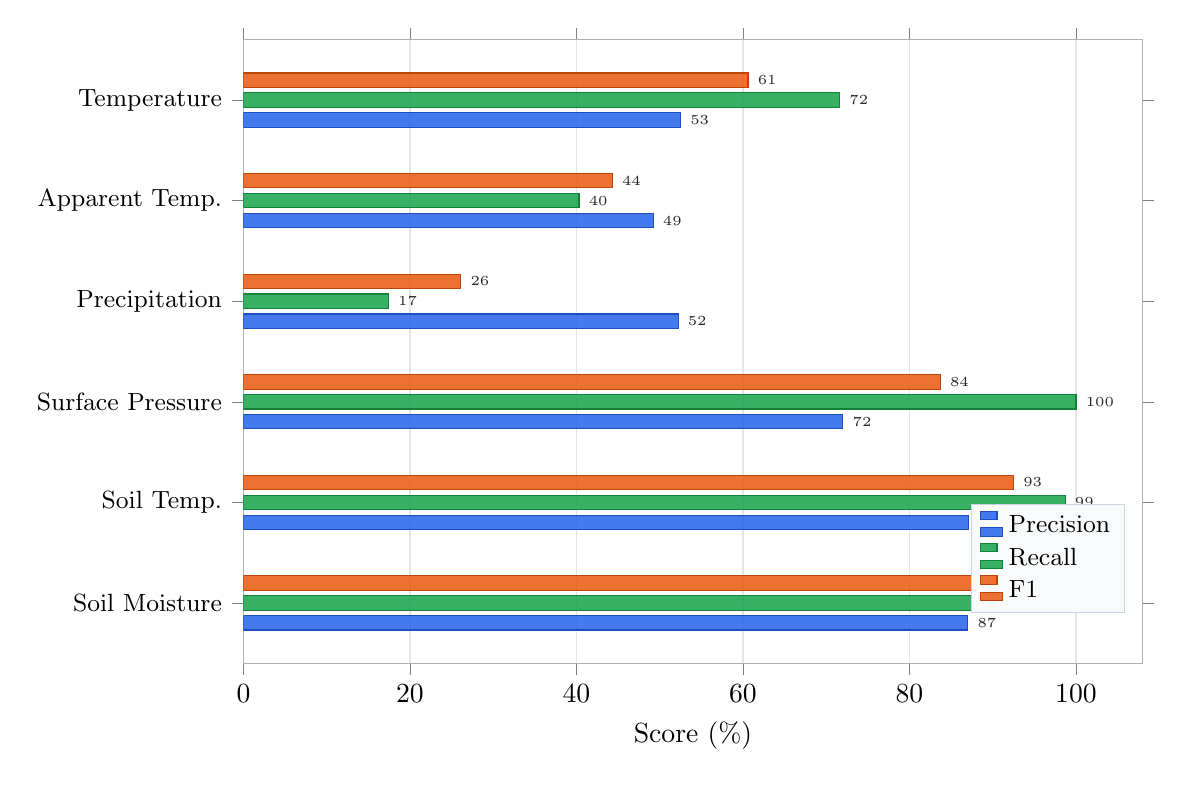
\begin{tikzpicture}
\begin{axis}[
  xbar,
  width=13cm, height=9.5cm,
  bar width=5.2pt,
  xmin=0, xmax=108,
  xlabel={Score (\%)},
  symbolic y coords={
    Soil Moisture,
    Soil Temp.,
    Surface Pressure,
    Precipitation,
    Apparent Temp.,
    Temperature
  },
  ytick=data,
  yticklabel style={font=\small},
  legend style={at={(0.98,0.08)}, anchor=south east, font=\small,
                legend columns=1, draw=codeborder, fill=codebg},
  legend cell align=left,
  enlarge y limits=0.12,
  tick align=outside,
  axis line style={draw=gray!60},
  major grid style={draw=gray!20},
  xmajorgrids=true,
  xtick={0,20,40,60,80,100},
  nodes near coords,
  nodes near coords style={font=\tiny, /pgf/number format/.cd, fixed, precision=0},
]
% Precision bars
\addplot[xbar, fill=precision, fill opacity=0.85, draw=precision!80!black]
  coordinates {
    (87.0,Soil Moisture)
    (87.1,Soil Temp.)
    (72.0,Surface Pressure)
    (52.2,Precipitation)
    (49.2,Apparent Temp.)
    (52.5,Temperature)
  };
% Recall bars
\addplot[xbar, fill=recall, fill opacity=0.85, draw=recall!80!black]
  coordinates {
    (94.4,Soil Moisture)
    (98.7,Soil Temp.)
    (100.0,Surface Pressure)
    (17.4,Precipitation)
    (40.3,Apparent Temp.)
    (71.6,Temperature)
  };
% F1 bars
\addplot[xbar, fill=f1color, fill opacity=0.85, draw=f1color!80!black]
  coordinates {
    (90.5,Soil Moisture)
    (92.5,Soil Temp.)
    (83.7,Surface Pressure)
    (26.1,Precipitation)
    (44.3,Apparent Temp.)
    (60.6,Temperature)
  };
\legend{Precision, Recall, F1}
\end{axis}
\end{tikzpicture}
\end{center}
\caption{Precision, recall, and F1 scores for Amsterdam detection across all six columns. Precision measures the share of raised flags that are real anomalies, recall measures the share of real anomalies that are detected, and F1 summarizes the balance between precision and recall.}
\label{fig:ams_bar}
\end{figure}

Recall matters more here: a missed anomaly silently corrupts downstream data, while a false alarm costs only a manual review.

\subsubsection{Model Selection Across All Cities}

Figure~\ref{fig:donut} shows which algorithm Optuna selected across all 30 trained models (5 cities $\times$ 6 columns). LOF was chosen in 80\% of cases and ECOD was selected for surface pressure in 4 out of 5 cities (Paris used HBOS instead).

\begin{figure}[!htbp]
\begin{center}
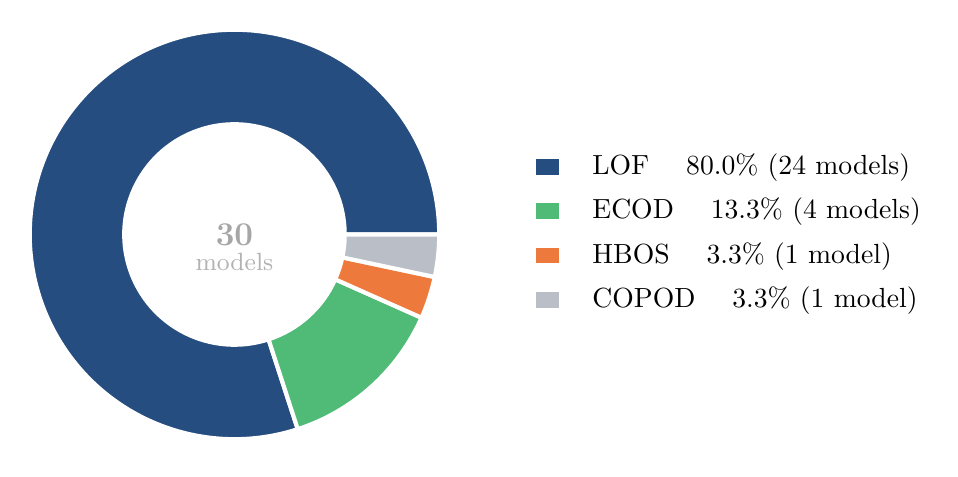
\begin{tikzpicture}
% LOF: 24/30 = 80.00% -> 288.0 degrees
% ECOD: 4/30 = 13.33% -> 48.0 degrees
% HBOS: 1/30 = 3.33%  -> 12.0 degrees
% COPOD: 1/30 = 3.33% -> 12.0 degrees
\def\R{2.6}   % outer radius
\def\r{1.4}   % inner radius

% LOF slice: 0 to 288.0 deg
\fill[leidenblue!85, draw=white, line width=1.5pt]
  (0,0) -- ({cos(0)*\R},{sin(0)*\R})
  arc[start angle=0, end angle=288.0, radius=\R]
  -- ({cos(288.0)*\r},{sin(288.0)*\r})
  arc[start angle=288.0, end angle=0, radius=\r]
  -- cycle;

% ECOD slice: 288.0 to 336.0 deg
\fill[recall!75, draw=white, line width=1.5pt]
  (0,0) -- ({cos(288.0)*\R},{sin(288.0)*\R})
  arc[start angle=288.0, end angle=336.0, radius=\R]
  -- ({cos(336.0)*\r},{sin(336.0)*\r})
  arc[start angle=336.0, end angle=288.0, radius=\r]
  -- cycle;

% HBOS slice: 336.0 to 348.0 deg
\fill[f1color!80, draw=white, line width=1.5pt]
  (0,0) -- ({cos(336.0)*\R},{sin(336.0)*\R})
  arc[start angle=336.0, end angle=348.0, radius=\R]
  -- ({cos(348.0)*\r},{sin(348.0)*\r})
  arc[start angle=348.0, end angle=336.0, radius=\r]
  -- cycle;

% COPOD slice: 348.0 to 360 deg
\fill[colorgray!70, draw=white, line width=1.5pt]
  (0,0) -- ({cos(348.0)*\R},{sin(348.0)*\R})
  arc[start angle=348.0, end angle=360, radius=\R]
  -- ({cos(360)*\r},{sin(360)*\r})
  arc[start angle=360, end angle=348.0, radius=\r]
  -- cycle;

% Centre label
\node[font=\bfseries\large, text=gray!70] at (0,0) {30};
\node[font=\small, text=gray!60] at (0,-0.35) {models};

% Legend placed to the right using node
\node[anchor=west, xshift=0.5cm] at (3.2,0) {%
  \begin{tabular}{@{}ll@{}}
    \tikz\fill[leidenblue!85] (0,0) rectangle (0.3,0.2); & LOF \quad 80.0\% (24 models)\\[4pt]
    \tikz\fill[recall!75] (0,0) rectangle (0.3,0.2);     & ECOD \quad 13.3\% (4 models)\\[4pt]
    \tikz\fill[f1color!80] (0,0) rectangle (0.3,0.2);    & HBOS \quad 3.3\% (1 model)\\[4pt]
    \tikz\fill[colorgray!70] (0,0) rectangle (0.3,0.2);  & COPOD \quad 3.3\% (1 model)\\
  \end{tabular}
};
\end{tikzpicture}
\end{center}
\caption{Algorithm selected by Optuna across all 30 trained models (5 cities $\times$ 6 columns). LOF was selected in 80\% of cases. ECOD was selected for the surface pressure column in 4 out of 5 cities (Paris used HBOS).}
\label{fig:donut}
\end{figure}

\subsubsection{Multi-City Comparison}

Figure~\ref{fig:multicity} highlights three representative columns across all five cities: surface pressure (best performing), soil moisture (consistently high), and temperature (most variable). Figure~\ref{fig:multicity_full} extends this to all six columns, ordered by average F2 from lowest to highest.

\begin{figure}[!htbp]
\begin{center}
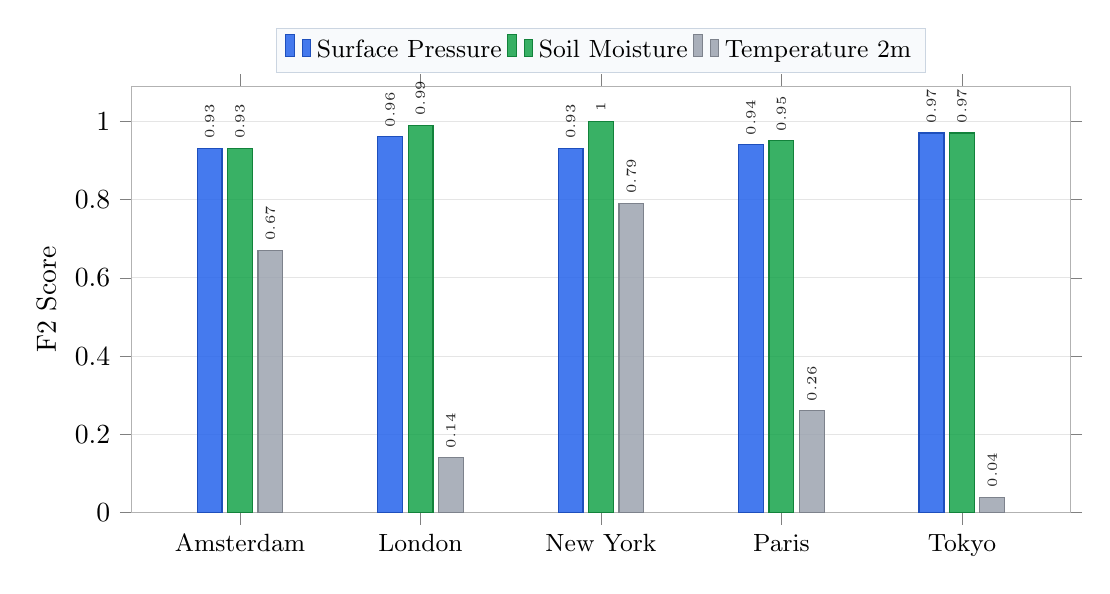
\begin{tikzpicture}
\begin{axis}[
  ybar,
  width=13.5cm, height=7cm,
  bar width=9pt,
  ymin=0, ymax=1.09,
  ylabel={F2 Score},
  symbolic x coords={Amsterdam, London, New York, Paris, Tokyo},
  xtick=data,
  xticklabel style={font=\small},
  legend style={at={(0.5,1.03)}, anchor=south, font=\small,
                legend columns=3, draw=codeborder, fill=codebg},
  legend cell align=left,
  enlarge x limits=0.15,
  tick align=outside,
  axis line style={draw=gray!60},
  ymajorgrids=true,
  major grid style={draw=gray!20},
  ytick={0,0.2,0.4,0.6,0.8,1.0},
  yticklabel={\pgfmathprintnumber[fixed,precision=1]{\tick}},
  nodes near coords,
  nodes near coords style={font=\tiny, rotate=90, anchor=west,
    /pgf/number format/.cd, fixed, precision=2},
]
% Surface pressure F2
\addplot[fill=precision, fill opacity=0.85, draw=precision!80!black]
  coordinates {
    (Amsterdam, 0.93)
    (London,    0.96)
    (New York,  0.93)
    (Paris,     0.94)
    (Tokyo,     0.97)
  };
% Soil moisture F2
\addplot[fill=recall, fill opacity=0.85, draw=recall!80!black]
  coordinates {
    (Amsterdam, 0.93)
    (London,    0.99)
    (New York,  1.00)
    (Paris,     0.95)
    (Tokyo,     0.97)
  };
% Temperature F2
\addplot[fill=colorgray, fill opacity=0.85, draw=colorgray!80!black]
  coordinates {
    (Amsterdam, 0.67)
    (London,    0.14)
    (New York,  0.79)
    (Paris,     0.26)
    (Tokyo,     0.04)
  };
\legend{Surface Pressure, Soil Moisture, Temperature 2m}
\end{axis}
\end{tikzpicture}
\end{center}
\caption{F2 scores across all five cities for three representative columns. Surface pressure and soil moisture are consistently high across all cities. Temperature detection varies significantly, suggesting that local climate variability and the column's noise level strongly influence difficulty.}
\label{fig:multicity}
\end{figure}

\begin{figure}[!htbp]
\begin{center}
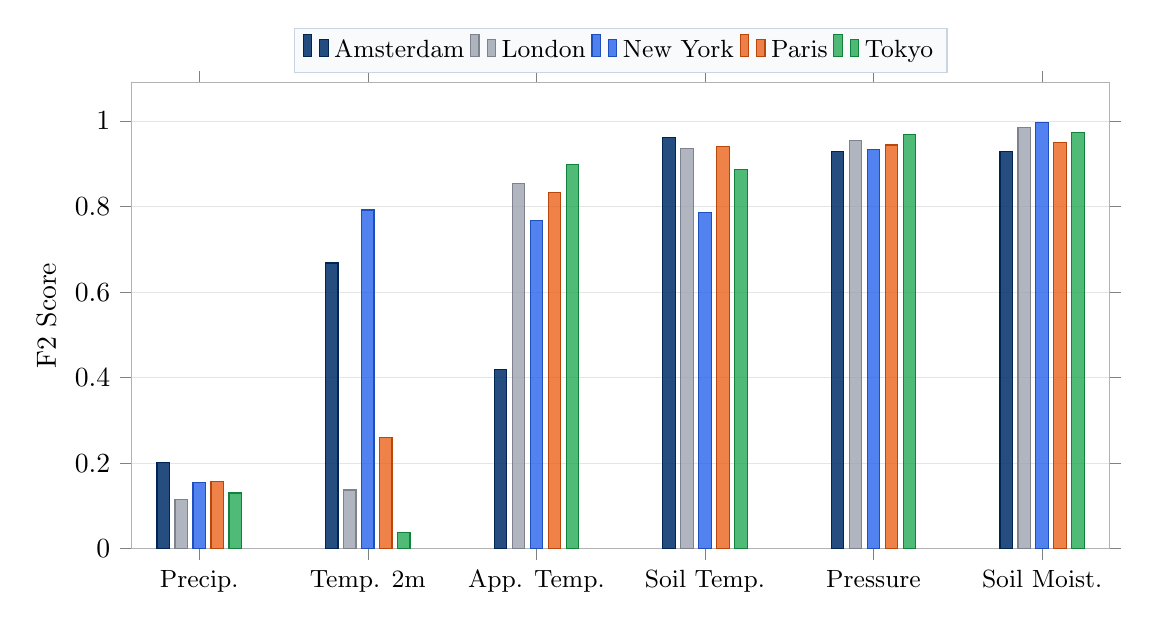
\begin{tikzpicture}
\begin{axis}[
  ybar,
  width=14cm, height=7.5cm,
  bar width=4.5pt,
  ymin=0, ymax=1.09,
  ylabel={F2 Score},
  symbolic x coords={
    {Precip.},
    {Temp. 2m},
    {App. Temp.},
    {Soil Temp.},
    {Pressure},
    {Soil Moist.}
  },
  xtick=data,
  xticklabel style={font=\small},
  legend style={at={(0.5,1.02)}, anchor=south, font=\small,
                legend columns=5, draw=codeborder, fill=codebg},
  legend cell align=left,
  enlarge x limits=0.08,
  tick align=outside,
  axis line style={draw=gray!60},
  ymajorgrids=true,
  major grid style={draw=gray!20},
  ytick={0, 0.2, 0.4, 0.6, 0.8, 1.0},
  yticklabel={\pgfmathprintnumber[fixed,precision=1]{\tick}},
]
\addplot[fill=leidenblue,  fill opacity=0.85, draw=leidenblue!80!black]
  coordinates {({Precip.},0.201) ({Temp. 2m},0.668) ({App. Temp.},0.418)
               ({Soil Temp.},0.961) ({Pressure},0.928) ({Soil Moist.},0.928)};
\addplot[fill=colorgray,   fill opacity=0.80, draw=colorgray!80!black]
  coordinates {({Precip.},0.115) ({Temp. 2m},0.137) ({App. Temp.},0.855)
               ({Soil Temp.},0.936) ({Pressure},0.955) ({Soil Moist.},0.985)};
\addplot[fill=precision,   fill opacity=0.80, draw=precision!80!black]
  coordinates {({Precip.},0.154) ({Temp. 2m},0.792) ({App. Temp.},0.768)
               ({Soil Temp.},0.787) ({Pressure},0.934) ({Soil Moist.},0.997)};
\addplot[fill=f1color,     fill opacity=0.75, draw=f1color!80!black]
  coordinates {({Precip.},0.157) ({Temp. 2m},0.259) ({App. Temp.},0.833)
               ({Soil Temp.},0.941) ({Pressure},0.944) ({Soil Moist.},0.949)};
\addplot[fill=recall,      fill opacity=0.75, draw=recall!80!black]
  coordinates {({Precip.},0.130) ({Temp. 2m},0.038) ({App. Temp.},0.898)
               ({Soil Temp.},0.887) ({Pressure},0.968) ({Soil Moist.},0.973)};
\legend{Amsterdam, London, {New York}, Paris, Tokyo}
\end{axis}
\end{tikzpicture}
\end{center}
\caption{F2 scores across all five cities and all six columns, ordered by average F2 from left to right. Precipitation is consistently low across all cities. Apparent temperature and temperature vary by city. Soil and pressure columns are reliably high everywhere, making them the strongest candidates for adaptive profiling.}
\label{fig:multicity_full}
\end{figure}

\subsubsection{Shift Magnitude vs. Detection Rate}

Figure~\ref{fig:shift} shows how detection rate changes with the size of the injected shift, measured as a percentage of the column's natural value range.

\begin{figure}[!htbp]
\begin{center}
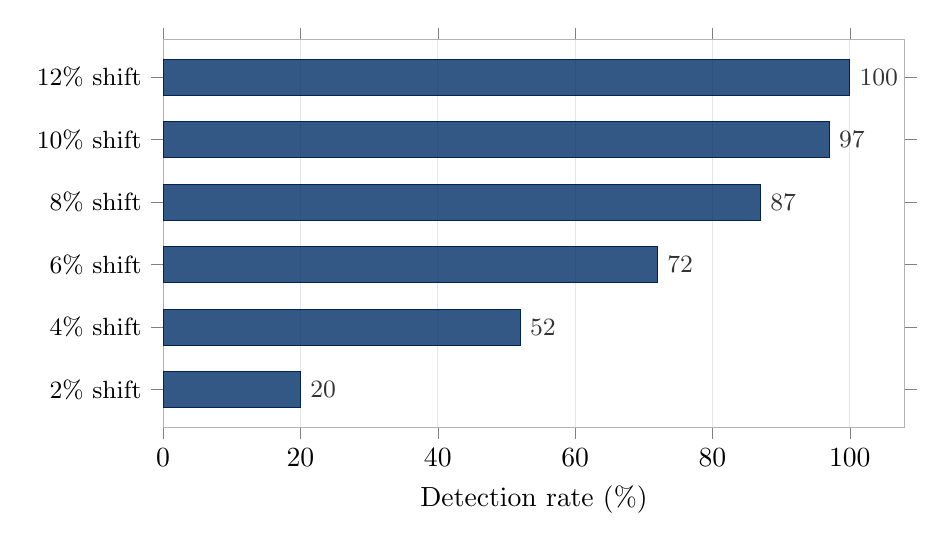
\begin{tikzpicture}
\begin{axis}[
  xbar,
  width=11cm, height=6.5cm,
  bar width=13pt,
  xmin=0, xmax=108,
  xlabel={Detection rate (\%)},
  ytick={1,2,3,4,5,6},
  yticklabels={2\% shift, 4\% shift, 6\% shift, 8\% shift, 10\% shift, 12\% shift},
  yticklabel style={font=\small},
  tick align=outside,
  axis line style={draw=gray!60},
  xmajorgrids=true,
  major grid style={draw=gray!20},
  xtick={0,20,40,60,80,100},
  enlarge y limits=0.12,
  nodes near coords,
  nodes near coords style={font=\small, /pgf/number format/.cd, fixed, precision=0},
]
\addplot[xbar, fill=leidenblue, fill opacity=0.80, draw=leidenblue!80!black]
  coordinates {(20,1) (52,2) (72,3) (87,4) (97,5) (100,6)};
\end{axis}
\end{tikzpicture}
\end{center}
\caption{Detection rate by injected shift size for Amsterdam temperature (univariate LOF). The shift is expressed as a percentage of the column's natural value range. Very small anomalies (2\%) are hard to distinguish from normal variation. Anomalies of 10\% or more are caught reliably.}
\label{fig:shift}
\end{figure}

\subsubsection{Generalization to Electricity Data}
\label{sec:elec_generalization}

To verify that the approach generalizes beyond weather data, we applied the Adaptive Profiler to GB national electricity demand records from the Elexon BMRS Insights API \cite{elexonbmrs2026}. The dataset contains two columns: \texttt{initialDemandOutturn} (INDO) and \texttt{initialTransmissionSystemDemandOutturn} (ITSDO). We injected 147 synthetic anomalies at a rate of 2.00\%, with shifts of 50--100\% of the original value distributed randomly in sign and target column.

This experiment was conducted by running the profiler twice on the same data. The untuned run is equivalent to \texttt{automl: true} with default hyperparameters in \texttt{profiling\_schema.yml} selected by Optuna. The tuned run has customized parameters found by the script to fit better based on data characteristics and ground truth, simulating a data engineer setup for increasing detector accuracy. Table~\ref{tab:elec_before_after} shows the impact of tuning.

\begin{table}[H]
\begin{center}
{\footnotesize
\setlength{\tabcolsep}{4pt}
\begin{tabular}{@{}l r r r r r r@{}}
\toprule
Column & \multicolumn{3}{c}{Untuned baseline} & \multicolumn{3}{c}{Tuned AutoML} \\
\cmidrule(lr){2-4}\cmidrule(lr){5-7}
 & Model & F2 & Recall & Model & F2 & Recall \\
\midrule
INDO  & IForest & 0.769 & 0.835 & HBOS & 0.929 & 0.961 \\
ITSDO & IForest & 0.788 & 0.924 & ECOD & 0.902 & 0.911 \\
\bottomrule
\end{tabular}
}
\end{center}
\caption{F2 and recall before and after AutoML tuning on GB electricity demand.}
\label{tab:elec_before_after}
\end{table}

Table~\ref{tab:elec_detection} shows the detection breakdown for the tuned run. Missed rates stay below 9\% for both columns.

\begin{table}[H]
\begin{center}
\begin{tabular}{@{}l r r r r r@{}}
\toprule
Column & Synthetic & Caught & Missed rate & Extra flags & FP rate \\
\midrule
INDO  & 103 & 99 & 3.9\% & 22 & 0.30\% \\
ITSDO & 79  & 72 & 8.9\% & 11 & 0.15\% \\
\bottomrule
\end{tabular}
\end{center}
\caption{Detection breakdown for the tuned AutoML run on GB electricity demand. Extra flags are non-synthetic rows scored as anomalous by the model.}
\label{tab:elec_detection}
\end{table}

\begin{figure}[H]
  \begin{center}
  \includegraphics[width=\textwidth]{images/elec_indo_scatter}
  \end{center}
  \caption{Detection overlay for GB initial demand outturn (INDO). Green rings are detected synthetic anomalies, purple rings are missed anomalies, and orange diamonds are extra flags on non-synthetic records (22 flags, 0.30\% FP rate). The tuned HBOS model catches 99 of 103 injected anomalies.}
  \label{fig:elec_indo_scatter}
\end{figure}

\begin{figure}[H]
  \begin{center}
  \includegraphics[width=\textwidth]{images/elec_itsdo_scatter}
  \end{center}
  \caption{Detection overlay for GB transmission system demand outturn (ITSDO). The tuned ECOD model catches 72 of 79 injected anomalies (purple rings mark the 7 missed). The 7 missed anomalies occur near the period of seasonal demand decline, where the local contrast used for scoring is reduced.}
  \label{fig:elec_itsdo_scatter}
\end{figure}

\paragraph{Shift magnitude vs.\ detection rate.}
Figure~\ref{fig:elec_shift} compares detection rate by shift band for INDO. At the 50--60\% band the tuned model detects 95\% of anomalies versus 67\% for the untuned baseline, both reach 100\% at shifts of 80\% or above. The benefit of tuning is largest where the signal is weakest.

\begin{figure}[H]
\begin{center}
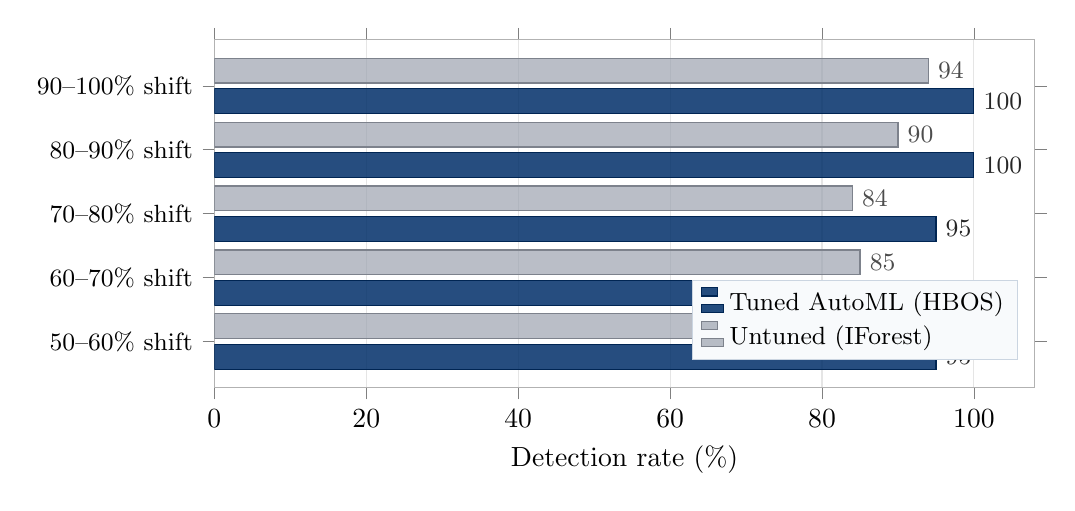
\begin{tikzpicture}
\begin{axis}[
  xbar,
  width=12cm, height=6cm,
  bar width=9pt,
  xmin=0, xmax=108,
  xlabel={Detection rate (\%)},
  ytick={1,2,3,4,5},
  yticklabels={50--60\% shift, 60--70\% shift, 70--80\% shift,
               80--90\% shift, 90--100\% shift},
  yticklabel style={font=\small},
  tick align=outside,
  axis line style={draw=gray!60},
  xmajorgrids=true,
  major grid style={draw=gray!20},
  xtick={0,20,40,60,80,100},
  enlarge y limits=0.18,
  nodes near coords,
  nodes near coords style={font=\small, /pgf/number format/.cd, fixed, precision=0},
  legend style={at={(0.98,0.08)}, anchor=south east, font=\small,
                draw=codeborder, fill=codebg},
  legend cell align=left,
]
\addplot[xbar, fill=leidenblue, fill opacity=0.85, draw=leidenblue!80!black]
  coordinates {(95,1) (92,2) (95,3) (100,4) (100,5)};
\addplot[xbar, fill=colorgray,  fill opacity=0.70, draw=colorgray!80!black]
  coordinates {(67,1) (85,2) (84,3) (90,4) (94,5)};
\legend{Tuned AutoML (HBOS), Untuned (IForest)}
\end{axis}
\end{tikzpicture}
\end{center}
\caption{Detection rate by injected shift size for INDO (tuned AutoML vs.\ untuned IForest baseline). Anomalies at 80\% shift or above are caught by both approaches. The tuned run provides the largest benefit at the 50--60\% shift band, lifting detection from 67\% to 95\%.}
\label{fig:elec_shift}
\end{figure}

\subsection{Experiment 2: Practical Overhead and Scaling}

The second experiment answers the second research sub-question: is ML-based profiling practical in terms of pipeline overhead and resource usage?

A built-in projection tool in the profiling library benchmarks training time across different data sizes, column counts, and trial budgets, then fits an empirical scaling law to the results. We ran it across approximately 90 benchmark configurations on the same hardware used for production. This tool lets any user predict how long training will take at their full data scale before committing to a deployment.

\subsubsection{The Scaling Formula}

The formula is inspired by work in ML research showing that training behavior follows power laws. Kaplan et al.\ \cite{kaplan2020scalinglawsneurallanguage} showed that for the majority of AI models, training performance scales predictably with data size, model size, and compute. Each factor contributes independently, so they can be multiplied together. The result has the shape: \emph{training performance = constant $\times$ (data size)$^\text{exponent}$ $\times$ (model size)$^\text{exponent}$}. Bordelon et al.\ \cite{pmlr-v235-bordelon24a} later showed theoretically that training time, data size, and model size each carry their own power-law exponent, and those exponents can differ from each other.

The formula uses the same structure where inputs are rows ($n$), columns ($m$), and Optuna trials ($k$). Hardware power directly affects the $\alpha$ constant across all benchmark runs. The fitted formula is:

$$T(n,\, m,\, k) \;=\; \alpha \cdot n^{\,\beta} \cdot m^{\,\delta} \cdot k^{\,\gamma}$$

Table~\ref{tab:scaling_params} explains what each symbol means and where its value comes from.

\begin{table}[H]
\begin{center}
\begin{tabularx}{\linewidth}{@{}llX@{}}
\toprule
Symbol & Name & Definition \\
\midrule
$n$      & Rows              & Number of records used for training \\
$m$      & Columns           & Number of features to be profiled having \texttt{automl: true} \\
$k$      & Trials            & Amount of models and parameters Optuna tries \\
\midrule
$\alpha$ & Baseline constant & Fitted from benchmark runs and depends on the hardware \\
$\beta$  & Row exponent      & Fitted by benchmarking at different row counts \\
$\delta$ & Column exponent   & Fitted by benchmarking at different column counts \\
$\gamma$ & Trial exponent    & Fitted by benchmarking at different trial counts \\
\bottomrule
\end{tabularx}
\end{center}
\caption{Inputs and fitted parameters. $n$, $m$, $k$ are known at runtime. The exponents $\beta$, $\delta$, $\gamma$ describe how time scales with each factor and primarily reflect algorithmic scaling rather than hardware. $\alpha$ is hardware-dependent and was fitted on the benchmark machine.}
\label{tab:scaling_params}
\end{table}

The exponents $\beta$, $\delta$, $\gamma$ primarily reflect properties of the algorithms and data structure rather than hardware, while $\alpha$ captures most of the hardware-dependent variation across machines. On substantially different systems the exponents may need refitting. All four values can only be obtained by running the projection tool across different configurations and measuring real training times.

\subsubsection{Scaling Behavior Depends on Algorithm Choice}

The key exponent is $\beta$, which controls how training time grows as the dataset gets larger. Table~\ref{tab:beta_meaning} shows what different values of $\beta$ mean in practice.

\begin{table}[!htbp]
\begin{center}
\begin{tabular}{@{}lll@{}}
\toprule
$\beta$ value & Scaling behavior & Effect of doubling the data \\
\midrule
$= 1.0$ & Linear      & Training time also doubles \\
$< 1.0$ & Sub-linear  & Training time grows slower than the data \\
$> 1.0$ & Super-linear & Training time grows faster than the data \\
\midrule
\textit{IForest (best):} $0.307$ & Sub-linear  & Doubled data took $1.24\times$ more time \\
\bottomrule
\end{tabular}
\end{center}
\caption{What different values of $\beta$ mean for how training time scales with data size.}
\label{tab:beta_meaning}
\end{table}

Figure~\ref{fig:train_scaling} shows per-algorithm training time projections. The fitted $\beta$ values span from 0.307 (IForest, sub-linear) to 1.175 (LOF, super-linear). The key finding is that \textbf{algorithm choice determines scaling behavior more than data size alone}.

\begin{figure}[H]
\begin{center}
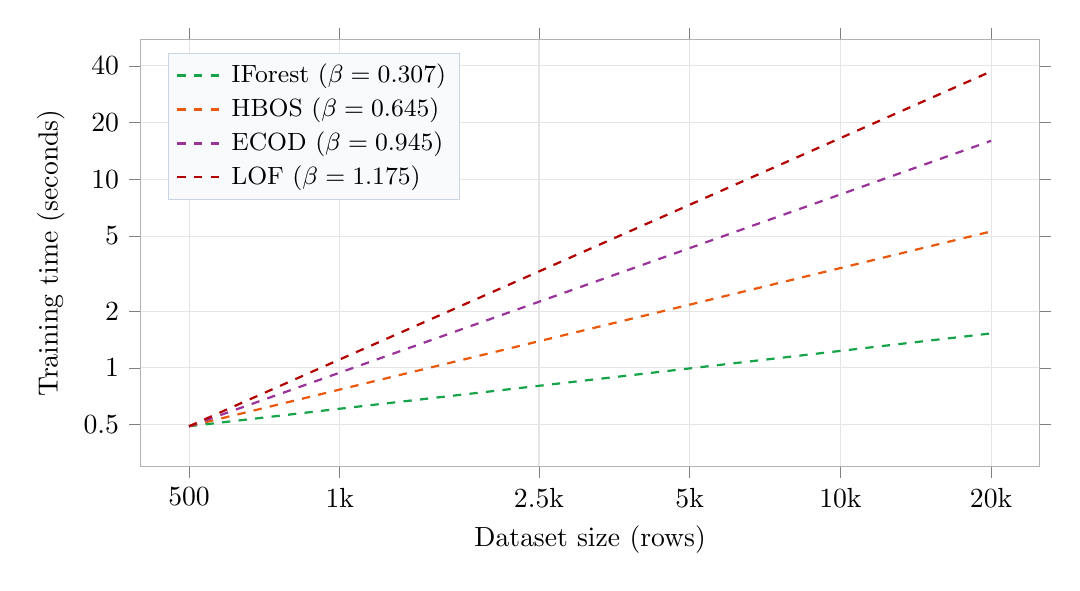
\begin{tikzpicture}
\begin{axis}[
  width=13cm, height=7cm,
  xlabel={Dataset size (rows)},
  ylabel={Training time (seconds)},
  xmode=log, ymode=log,
  xmin=400, xmax=25000,
  ymin=0.3, ymax=55,
  xtick={500,1000,2500,5000,10000,20000},
  xticklabels={500, 1k, 2.5k, 5k, 10k, 20k},
  ytick={0.5,1,2,5,10,20,40},
  yticklabels={0.5, 1, 2, 5, 10, 20, 40},
  tick align=outside,
  axis line style={draw=gray!60},
  ymajorgrids=true,
  xmajorgrids=true,
  major grid style={draw=gray!20},
  legend style={at={(0.03,0.97)}, anchor=north west, font=\small,
                draw=codeborder, fill=codebg, legend columns=1},
  legend cell align=left,
]
% IForest projection
\addplot[color=recall, dashed, thick]
  coordinates {(500,0.490)(1000,0.607)(2500,0.803)(5000,0.993)(10000,1.230)(20000,1.523)};
\addlegendentry{IForest ($\beta=0.307$)}
% HBOS projection
\addplot[color=f1color, dashed, thick]
  coordinates {(500,0.490)(1000,0.767)(2500,1.384)(5000,2.164)(10000,3.383)(20000,5.292)};
\addlegendentry{HBOS ($\beta=0.645$)}
% ECOD projection
\addplot[color=violet!80, dashed, thick]
  coordinates {(500,0.490)(1000,0.943)(2500,2.242)(5000,4.317)(10000,8.315)(20000,16.01)};
\addlegendentry{ECOD ($\beta=0.945$)}
% LOF projection
\addplot[color=red!70!black, dashed, thick]
  coordinates {(500,0.490)(1000,1.108)(2500,3.247)(5000,7.330)(10000,16.55)(20000,37.37)};
\addlegendentry{LOF ($\beta=1.175$)}
\end{axis}
\end{tikzpicture}
\end{center}
\caption{Per-algorithm training time projections on a log-log scale, anchored at the same starting point (500 rows). Steeper slope indicates higher $\beta$. LOF is the only super-linear algorithm.}
\label{fig:train_scaling}
\end{figure}

Table~\ref{tab:multipliers} shows the effect of $\beta$ on scaling for each algorithm when data size grows.

\begin{table}[H]
\begin{center}
\begin{tabular}{@{}llll@{}}
\toprule
Algorithm & $\beta$ & $2\times$ data & $10\times$ data \\
\midrule
IForest  & 0.307 & $1.24\times$ more time & $2.03\times$ more time \\
HBOS     & 0.645 & $1.56\times$ more time & $4.42\times$ more time \\
ECOD     & 0.945 & $1.93\times$ more time & $8.81\times$ more time \\
LOF      & 1.175 & $2.26\times$ more time & $14.96\times$ more time \\
\bottomrule
\end{tabular}
\end{center}
\caption{How training time multiplies when data grows, per algorithm.}
\label{tab:multipliers}
\end{table}

\subsubsection{Per-Algorithm Scaling}

Figure~\ref{fig:beta_chart} summarizes the fitted $\beta$ per algorithm. IForest is the most scalable. LOF is the only super-linear algorithm.

\begin{figure}[H]
\begin{center}
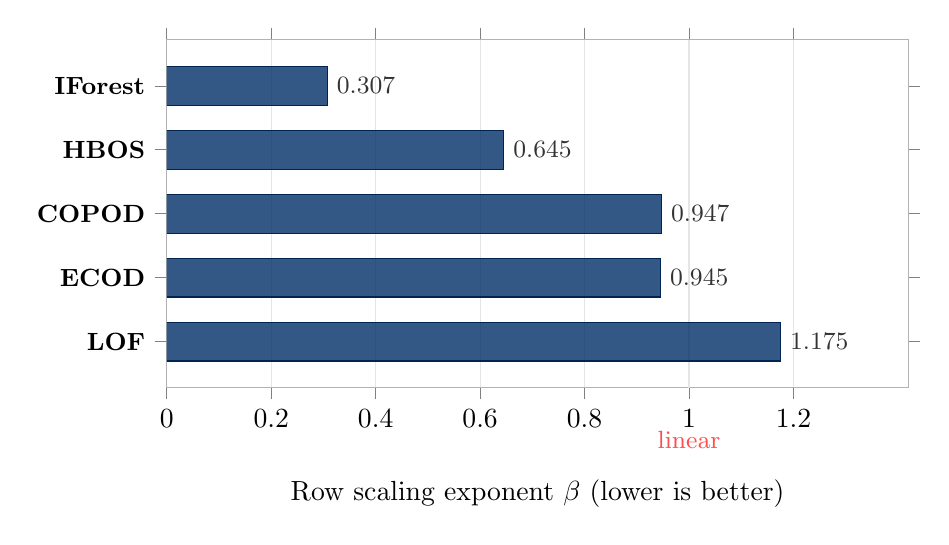
\begin{tikzpicture}
\begin{axis}[
  xbar,
  width=11cm, height=6cm,
  bar width=14pt,
  xmin=0, xmax=1.42,
  xlabel={Row scaling exponent $\beta$ (lower is better)},
  symbolic y coords={LOF, ECOD, COPOD, HBOS, IForest},
  ytick=data,
  yticklabel style={font=\small\bfseries},
  tick align=outside,
  axis line style={draw=gray!60},
  xmajorgrids=true,
  major grid style={draw=gray!20},
  xtick={0, 0.2, 0.4, 0.6, 0.8, 1.0, 1.2},
  enlarge y limits=0.18,
  nodes near coords,
  nodes near coords style={font=\small, /pgf/number format/.cd, fixed, precision=3},
  % reference line at beta=1
  extra x ticks={1.0},
  extra x tick style={
    grid=major,
    grid style={dashed, red!60, line width=0.8pt},
    tick style={draw=none},
    xticklabel={\small linear},
    xticklabel style={red!70, yshift=-8pt},
  },
]
\addplot[
  xbar,
  fill={leidenblue},
  fill opacity=0.80,
  draw=leidenblue!80!black,
] coordinates {
  (1.175,LOF)
  (0.945,ECOD)
  (0.947,COPOD)
  (0.645,HBOS)
  (0.307,IForest)
};
\end{axis}
% "super-linear" annotation
\end{tikzpicture}
\end{center}
\caption{Fitted row scaling exponent $\beta$ per algorithm from ~90 benchmark observations.}
\label{fig:beta_chart}
\end{figure}

\subsection{Experiment 3: AutoML vs.\ Neural Architecture Search}\label{sec:autonn_comparison}

To validate the choice of classical PyOD algorithms over neural network detectors, we ran both approaches on the same five-city dataset, same preprocessing, and same unsupervised objective. Neither sees anomaly labels at any point.

\begin{itemize}
  \item \textbf{AutoML:} Optuna selects among IForest, LOF, ECOD, HBOS, and COPOD with 25 trials per column.
  \item \textbf{Auto-NN:} Optuna performs neural architecture search (NAS) over two neural network models, the Autoencoder (AE) and Variational Autoencoder (VAE). It varies hidden layer count, width, activation function, learning rate, epoch count, and batch size, with 25 trials per column (matching AutoML for a direct comparison). One-Class SVM is intentionally excluded because it is not a neural network.
\end{itemize}

\subsubsection{Detection Results}

Table~\ref{tab:autonn_summary} and Figure~\ref{fig:autonn_compare} summarize the outcome. AutoML scored higher in 29 of 30 univariate cases and won decisively (margin $> 0.02$) in 27 of those 30. The three near-ties are: London surface pressure (AutoML 0.955 vs.\ Auto-NN 0.935, margin 0.020), New York surface pressure (AutoML 0.934 vs.\ Auto-NN 0.942, where Auto-NN leads by 0.008), and Tokyo temperature (AutoML 0.038 vs.\ Auto-NN 0.027, margin 0.011 with both models scoring very low). In the remaining 27 cases AutoML is decisively ahead, and it runs 9.13$\times$ faster overall on the same trial budget (same 25 trials).


\begin{table}[H]
\begin{center}
\begin{tabular}{@{}lcc@{}}
\toprule
Metric & AutoML & Auto-NN (AE/VAE) \\
\midrule
Mean F2 (univariate)        & \textbf{0.683} & 0.167 \\
Mean Recall                 & \textbf{0.765} & 0.196 \\
Mean Precision              & \textbf{0.618} & 0.153 \\
Mean total time / column    & \textbf{2.92 s} & 26.69 s \\
\bottomrule
\end{tabular}
\end{center}
\caption{AutoML vs.\ Auto-NN aggregate results across 5 cities $\times$ 6 columns.}
\label{tab:autonn_summary}
\end{table}

\begin{figure}[!htbp]
\begin{center}
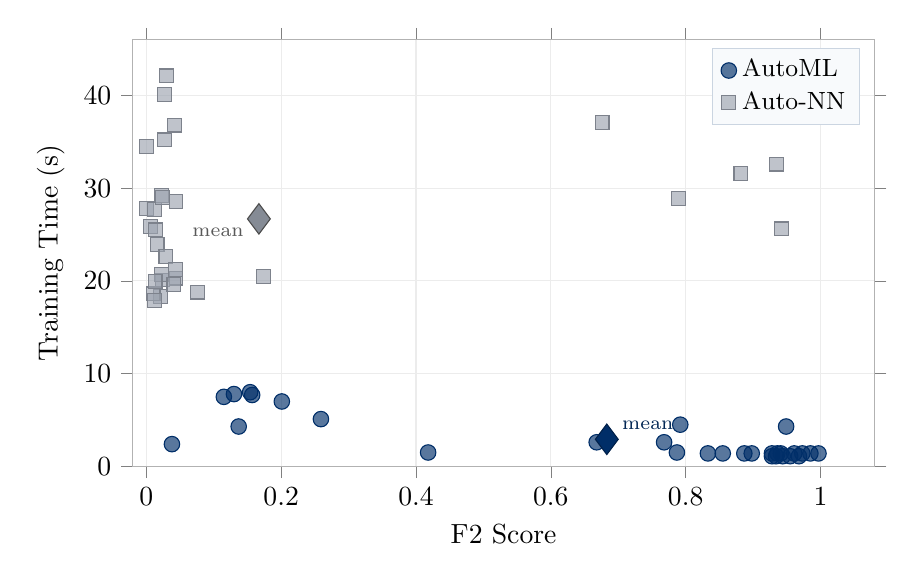
\begin{tikzpicture}
\begin{axis}[
  width=11cm, height=7cm,
  xlabel={F2 Score},
  ylabel={Training Time (s)},
  xmin=-0.02, xmax=1.08,
  ymin=0, ymax=46,
  xtick={0, 0.2, 0.4, 0.6, 0.8, 1.0},
  ytick={0, 10, 20, 30, 40},
  tick align=outside,
  axis line style={draw=gray!60},
  ymajorgrids=true,
  xmajorgrids=true,
  major grid style={draw=gray!15},
  legend style={at={(0.98,0.98)}, anchor=north east, font=\small,
                draw=codeborder, fill=codebg},
  legend cell align=left,
]
%% AutoML — one point per city/column pair
\addplot[only marks, mark=*, mark size=2.8pt,
  mark options={fill=leidenblue, fill opacity=0.65, draw=leidenblue}]
  coordinates {
    (0.418,1.5)  (0.201,7.0)  (0.928,1.4)  (0.961,1.4)  (0.928,1.1)  (0.668,2.6)
    (0.855,1.4)  (0.115,7.5)  (0.985,1.4)  (0.936,1.4)  (0.955,1.1)  (0.137,4.3)
    (0.768,2.6)  (0.154,8.0)  (0.997,1.4)  (0.787,1.5)  (0.934,1.1)  (0.792,4.5)
    (0.833,1.4)  (0.157,7.7)  (0.949,4.3)  (0.941,1.4)  (0.944,1.1)  (0.259,5.1)
    (0.898,1.4)  (0.130,7.8)  (0.973,1.4)  (0.887,1.4)  (0.968,1.1)  (0.038,2.4)
  };
\addlegendentry{AutoML}
%% Auto-NN — one point per city/column pair
\addplot[only marks, mark=square*, mark size=2.5pt,
  mark options={fill=colorgray, fill opacity=0.65, draw=colorgray!80!black}]
  coordinates {
    (0.006,25.9)  (0.000,27.8)  (0.174,20.5)  (0.044,20.3)  (0.882,31.6)  (0.027,40.1)
    (0.024,20.1)  (0.014,25.5)  (0.044,28.6)  (0.021,18.3)  (0.935,32.6)  (0.010,18.6)
    (0.000,34.5)  (0.016,23.9)  (0.029,22.6)  (0.043,21.2)  (0.942,25.6)  (0.022,20.7)
    (0.012,27.7)  (0.022,29.2)  (0.030,42.1)  (0.041,19.6)  (0.676,37.1)  (0.012,17.9)
    (0.024,29.0)  (0.013,19.9)  (0.042,36.8)  (0.076,18.8)  (0.789,28.9)  (0.027,35.2)
  };
\addlegendentry{Auto-NN}
%% Mean markers
\addplot[only marks, mark=diamond*, mark size=5.5pt,
  mark options={fill=leidenblue, draw=leidenblue!70!black}]
  coordinates {(0.683,2.92)};
\addplot[only marks, mark=diamond*, mark size=5.5pt,
  mark options={fill=colorgray!85!black, draw=gray!60!black}]
  coordinates {(0.167,26.69)};
%% Mean labels
\node[font=\scriptsize, text=leidenblue!80!black, anchor=south west, xshift=2pt]
  at (axis cs:0.683,2.92) {mean};
\node[font=\scriptsize, text=gray!70!black, anchor=north east, xshift=-2pt]
  at (axis cs:0.167,26.69) {mean};
\end{axis}
\end{tikzpicture}
\end{center}
\caption{F2 score vs.\ training time for all 30 models per approach (one point per city--column pair). AutoML models cluster bottom-right: high F2, low training time. Most Auto-NN models sit top-left: low F2, high training time. The five Auto-NN outliers with high F2 are surface pressure columns, where neural reconstruction is more competitive on quality but remains around $10\times$ slower than AutoML. Filled diamonds mark the mean of each approach.}
\label{fig:autonn_compare}
\end{figure}

Table~\ref{tab:autonn_full} shows the full per-city, per-column breakdown with measured search time for each approach.

\begin{table}[H]
\begin{center}
{\footnotesize
\setlength{\tabcolsep}{4pt}
\begin{tabular}{@{}l l c r r c r r@{}}
\toprule
City & Column
  & \multicolumn{3}{c}{AutoML}
  & \multicolumn{3}{c}{Auto-NN} \\
\cmidrule(lr){3-5}\cmidrule(lr){6-8}
  &  & Model & F2 & Time (s) & Model & F2 & Time (s) \\
\midrule
Amsterdam & App.\ Temp.  & LOF  & 0.418 &  1.5 & AE  & 0.006 & 25.9 \\
Amsterdam & Precip.      & LOF  & 0.201 &  7.0 & VAE & 0.000 & 27.8 \\
Amsterdam & Soil Moist.  & LOF  & 0.928 &  1.4 & VAE & 0.174 & 20.5 \\
Amsterdam & Soil Temp.   & LOF  & 0.961 &  1.4 & AE  & 0.044 & 20.3 \\
Amsterdam & Pressure     & ECOD & 0.928 &  1.1 & VAE & 0.882 & 31.6 \\
Amsterdam & Temp.\ 2m    & LOF  & 0.668 &  2.6 & VAE & 0.027 & 40.1 \\
\midrule
London    & App.\ Temp.  & LOF  & 0.855 &  1.4 & VAE & 0.024 & 20.1 \\
London    & Precip.      & LOF  & 0.115 &  7.5 & VAE & 0.014 & 25.5 \\
London    & Soil Moist.  & LOF  & 0.985 &  1.4 & AE  & 0.044 & 28.6 \\
London    & Soil Temp.   & LOF  & 0.936 &  1.4 & AE  & 0.021 & 18.3 \\
London    & Pressure     & ECOD & 0.955 &  1.1 & VAE & 0.935 & 32.6 \\
London    & Temp.\ 2m    & LOF  & 0.137 &  4.3 & AE  & 0.010 & 18.6 \\
\midrule
New York  & App.\ Temp.  & LOF  & 0.768 &  2.6 & VAE & 0.000 & 34.5 \\
New York  & Precip.      & LOF  & 0.154 &  8.0 & VAE & 0.016 & 23.9 \\
New York  & Soil Moist.  & LOF  & 0.997 &  1.4 & AE  & 0.029 & 22.6 \\
New York  & Soil Temp.   & LOF  & 0.787 &  1.5 & AE  & 0.043 & 21.2 \\
New York  & Pressure     & ECOD & 0.934 &  1.1 & AE  & 0.942 & 25.6 \\
New York  & Temp.\ 2m    & LOF  & 0.792 &  4.5 & AE  & 0.022 & 20.7 \\
\midrule
Paris     & App.\ Temp.  & LOF  & 0.833 &  1.4 & AE  & 0.012 & 27.7 \\
Paris     & Precip.      & LOF  & 0.157 &  7.7 & VAE & 0.022 & 29.2 \\
Paris     & Soil Moist.  & LOF  & 0.949 &  4.3 & VAE & 0.030 & 42.1 \\
Paris     & Soil Temp.   & LOF  & 0.941 &  1.4 & VAE & 0.041 & 19.6 \\
Paris     & Pressure     & HBOS & 0.944 &  1.1 & AE  & 0.676 & 37.1 \\
Paris     & Temp.\ 2m    & LOF  & 0.259 &  5.1 & AE  & 0.012 & 17.9 \\
\midrule
Tokyo     & App.\ Temp.  & LOF  & 0.898 &  1.4 & AE  & 0.024 & 29.0 \\
Tokyo     & Precip.      & LOF  & 0.130 &  7.8 & AE  & 0.013 & 19.9 \\
Tokyo     & Soil Moist.  & LOF  & 0.973 &  1.4 & AE  & 0.042 & 36.8 \\
Tokyo     & Soil Temp.   & LOF  & 0.887 &  1.4 & VAE & 0.076 & 18.8 \\
Tokyo     & Pressure     & ECOD & 0.968 &  1.1 & VAE & 0.789 & 28.9 \\
Tokyo     & Temp.\ 2m    & COPOD& 0.038 &  2.4 & AE  & 0.027 & 35.2 \\
\bottomrule
\end{tabular}
}
\end{center}
\caption{Full detection results across all cities.}
\label{tab:autonn_full}
\end{table}

% ============================================================
\section{Discussion}\label{sec:discussion}
% ============================================================

\subsection{Detection Effectiveness}

\textbf{Column characteristics determine performance.} Surface pressure and soil columns have tight, predictable distributions, so even small shifts are statistically unusual. Temperature is noisier due to seasonal variation, and some injected anomalies overlap with natural extreme values. Precipitation is the hardest column because it is heavily right-skewed (most hours have zero rain).

\textbf{When AutoML is not the right choice.} Figure~\ref{fig:ams_precipitation} shows Amsterdam precipitation which follows a heavily right-skewed distribution: most hours record zero rain, and the hours that do have rainfall are highly variable with no stable seasonal shape. A model trained on this column had difficulty distinguishing an injected anomaly from a naturally extreme value in this dataset, which explains the consistently low F2 scores for precipitation across all five cities in these experiments. Columns with this kind of distribution may not be good candidates for ML-based anomaly detection. Running the profiling pipeline on a data sample before production deployment lets a data engineer identify these columns early and set \texttt{automl: false} for them rather than spending trials on a model that is unlikely to converge to a useful threshold.

\begin{figure}[!htbp]
  \begin{center}
  \includegraphics[width=\textwidth]{images/ams_precip.png}
  \end{center}
  \caption{Amsterdam precipitation from Apr 2024 to Apr 2026. Most hours record zero rain and the rest are highly variable, leaving no stable pattern to learn. AutoML performed poorly on anomaly detection for this task due to the nature of this specific data.}
  \label{fig:ams_precipitation}
\end{figure}

\textbf{Why LOF was chosen most often.} LOF measures local density by comparing each value to its nearest neighbors in feature space. For univariate weather columns, this captures how isolated a value is within the distribution of recent readings. An injected shift lands in a sparse region of that distribution, far from typical values, and therefore receives a high anomaly score.

\textbf{Why ECOD was selected for surface pressure.} Atmospheric pressure stays within a very narrow range most of the time. ECOD scores each value by how far it sits in the tail of the observed distribution. An injected shift lands immediately in that tail, making it easy to flag. Figure~\ref{fig:pressure} shows Amsterdam surface pressure: injected anomalies fall clearly outside the normal pressure band. The same pattern held in 4 of the 5 cities. Paris used HBOS for surface pressure instead, though also achieving high recall.

\begin{figure}[!htbp]
  \begin{center}
  \includegraphics[width=\textwidth]{images/ams_surface_pressure}
  \end{center}
  \caption{Amsterdam surface pressure from Apr 2024 to Apr 2026 with AutoML. ECOD selected by Optuna achieves 100\% recall where all injected anomalies fall clearly outside the tight normal pressure band.}
  \label{fig:pressure}
\end{figure}

\textbf{Multi-city patterns.} Performance is consistent across cities for the well-structured columns (surface pressure, soil moisture), but highly variable for noisy ones like temperature. London and Tokyo show very low temperature F2 scores (0.14 and 0.04), while Amsterdam and New York are much higher (0.67 and 0.79). This suggests that temperature is harder to profile in climates with more erratic variation. In such cases, the decision threshold should be tuned on validation data to detect failure points while controlling false alarms.

\textbf{Electricity data confirms the same pattern.} The electricity benchmark (Section~\ref{sec:elec_generalization}) reaches F2 of 0.929 and 0.902 on INDO and ITSDO respectively, consistent with the high scores seen on stable weather columns such as surface pressure and soil moisture. Optuna selected HBOS and ECOD, the same algorithm families that excelled on tight, well-bounded distributions in the weather experiments. The before-and-after comparison isolates the value of the tuning step: the untuned IForest baseline produced extra-flag rates of 0.84--1.02\% while simultaneously missing more anomalies, whereas the tuned run cut the false-positive rate to 0.15--0.30\% and improved recall. The electricity anomaly shifts (50--100\% of the original value) are far larger than the weather injections (2--12\%), so the high recall across both runs is expected.

\textbf{Shift magnitude.} Detection reaches near 100\% for shifts of 10 to 12\% of the column's value range, and drops to around 50 to 70\% for smaller shifts of 4 to 6\%. This threshold is useful for deciding if the model is sensitive enough for a given use case.

\subsection{AutoML vs.\ Auto-NN}

Surface pressure is the column where neural reconstruction is most competitive, because its tight near-Gaussian distribution makes reconstruction error a relatively reliable anomaly score. The Tokyo temperature near-tie is not a genuine win for either approach, since both score below 0.04 on a column where precipitation-like noise makes any unsupervised model unreliable.

The results confirm that AutoML outperforms neural architecture search in 29 of 30 univariate cases. Classical detectors (LOF, ECOD, HBOS, and COPOD) are naturally better suited to this task. They compare each point to its local neighborhood or tail probability rather than learning a global reconstruction mapping, which is exactly what is needed to detect point anomalies embedded in seasonal patterns. Beyond the quality advantage, AutoML is 9.13$\times$ faster overall on the same trial budget, making it the clear practical choice for tabular ETL anomaly detection.

\subsection{Threshold Calibration and the False-Positive Trade-off}

\textbf{The model flags some normal data.} On top of detecting synthetic anomalies, the model also flags a number of normal records as anomalous. This happens when a real value is statistically rare in the training window, for example, an unusually cold week or an extreme but valid pressure reading. These records are not pipeline errors, but they fall outside the pattern the model learned from recent history.

\textbf{Raising the detection threshold reduces false positives for stable columns.} The profiler outputs a continuous anomaly probability score for every record. A data engineer can require a higher score before a flag is raised. For surface pressure, this reduces false positives by 59\% on average across all five cities while keeping recall above 80\%. Apparent temperature and soil temperature improve by 41 to 47\% under similar conditions.

\textbf{Threshold tuning does not help all columns.} For temperature in high-variability climates like London and Paris, the model assigns similar confidence scores to natural weather extremes and to injected anomalies, so raising the threshold cuts both equally and precision does not improve. Setting \texttt{automl: false} is the better option for those columns. Precipitation should be disabled across all cities since even at the best threshold F2 stays below 0.21.

\begin{table}[!htbp]
\centering
\begin{tabular}{@{}l l r r r r r@{}}
\toprule
Column & Model & \multicolumn{2}{c}{Default} & \multicolumn{2}{c}{After tuning} & FP \\
\cmidrule(lr){3-4}\cmidrule(lr){5-6}
 & & FP rate & F2 & FP rate & F2 & reduction \\
\midrule
Temperature 2m   & LOF  & 2.38\% & 0.379 & 1.20\% & 0.362 & 37\% \\
Apparent Temp.   & LOF  & 0.30\% & 0.754 & 0.15\% & 0.680 & 47\% \\
Soil Temp.       & LOF  & 0.13\% & 0.902 & 0.08\% & 0.780 & 41\% \\
Precipitation    & LOF  & 0.09\% & 0.151 & 0.00\% & 0.134 & 74\% \\
Surface Pressure & ECOD & 0.07\% & 0.946 & 0.02\% & 0.848 & 59\% \\
Soil Moisture    & LOF  & 0.05\% & 0.966 & 0.04\% & 0.855 & 16\% \\
\bottomrule
\end{tabular}
\caption{False-positive rate and F2 score before and after threshold tuning, averaged across all five cities, each with 20,352 hourly records. Tuned thresholds were determined after the experiment using a script that aimed to balance the false-positive rate and F2 score, with injected anomalies treated as ground truth.}
\label{tab:threshold_summary}
\end{table}

\subsection{Training on Big Data}

\textbf{Real pipelines hold far more data than models need.} A data source that has been running for years will have too many rows to retrain on every day. The Adaptive Profiler library lets engineers set a training window so only the most recent rows are used. A window of a few thousand rows is sufficient to learn stable patterns while keeping training time within the bounds shown in the scaling experiment.

\textbf{Scheduled retraining keeps detection accurate over time.} In Apache Airflow, the retraining step can be added as a recurring DAG task on any schedule. The profiler's training mode runs as a single command, so a weekly or monthly job is simple to set up alongside the ingestion pipeline. If the data source changes due to seasonal shifts, sensor recalibration, or an upstream update, the next retraining run picks up the change without any manual work.

\subsection{Limitations of the Evaluation}

The evaluation relies on synthetically injected anomalies. Real data quality problems may look different: they may be sustained drift rather than point anomalies, or they may affect multiple columns at once.

All experiments use weather data, which has strong seasonal patterns and relatively stable distributions. The approach may behave differently on other types of data such as financial transactions or IoT sensor streams with abrupt regime changes.

If anomalies already exist in the historical training data, the model will learn to treat them as normal. This is a fundamental limitation of unsupervised learning.

The approach trains one model per column independently. Anomalies that only appear as correlated shifts across multiple columns simultaneously would not be detected by this design.


% ============================================================
\section{Conclusions and Further Work}\label{sec:conclusions}
% ============================================================

\subsection{Conclusion}

This thesis investigated whether learning-based anomaly detection is a reliable, low-cost addition to rule-based quality checks in the ingestion layer of ETL pipelines. The experiments confirm that AutoML-based profiling is a practical complement to rule-based checks.

\textbf{Effectiveness.} Learning-based profiling detected semantic anomalies that rule-based checks cannot catch. On stable columns such as surface pressure and soil moisture, models trained on one city generalized to all five, achieving F2 scores from 0.93 to 1.00. On noisier columns like temperature, F2 varied widely from 0.04 to 0.79.

\textbf{Practicality.} Integrating the profiling step required minimal changes to the Airflow DAG. Training time grows slowly for algorithms such as Isolation Forest ($\beta = 0.307$), so the overhead stays manageable as data volume increases. LOF grew faster with larger datasets ($\beta = 1.175$), making algorithm choice important for large-scale use. The library is configured with one simple line per column, which keeps the production setup practical.

\textbf{Learning model.} Machine learning outperformed neural architecture search in 29 of 30 settings. AutoML ran 9.13$\times$ faster on average and achieved a 4.1$\times$ higher mean F2 score. Classical models are naturally better suited to point anomaly detection in tabular ETL data than deep models that overfit reconstruction rather than distribution shape.

Together, these results show that AutoML-based adaptive profiling can improve data quality for downstream users at a manageable cost. A small pilot on the target data before production deployment is enough to determine whether the approach is a good fit based on the nature of each column of upstream data.


\subsection{Further Work}

Evaluating the approach on datasets from domains such as finance, IoT, or e-commerce would establish how well it generalizes beyond weather data.

The evaluation used point anomalies in individual columns. Extending detection to joint anomalies would make predictions more robust and enable multivariate anomaly detection rather than limiting the tool to univariate use.

Adding automatic drift detection and retraining triggers would enable the system to adapt automatically when upstream source distributions change over time.

Exposing why a record was flagged would help engineers monitor model decisions and reason about AutoML behavior in production.

\bibliographystyle{plain}
\bibliography{bibliography}
\addcontentsline{toc}{section}{References}

\end{document}